% !TEX root = ../thesis.tex
% basics
% @author Tobias Wulf
%

\chapter{Grundlagen 0.0.2 19.02.2021}\label{ch:grundlagen}

Das Fundament für die Drehwinkelerfassung mittels magnetischen Sensor-Array und lernender Signalverarbeitung 
\cite{Schuethe2019}\cite{Schuethe2020a}\cite{Schuethe2020} bildet das Regressionsverfahren für Gauß-Prozesse 
\cite{Rasmussen2006} und die damit verbundene Abstandmessung von Winkelpositionen auf einer Kreisbahn.
Für eine anschauliche Erklärung der Grundlagen, sollen die Zusammenhänge anhand einfacher Kreisdarstellung des 
Messprinzips eines einzelnen Winkelsensors gezeigt werden. Sodass dieses später in der Verwendung eines Sensor-Arrays 
adaptierbar ist und mittels geeigneter Rechen- und Normierungsverfahren auf die Problemstellung eines 
höherdimensionalen Systems projiziert werden kann.


% !TEX root = ../thesis.tex
% circle view of angular application
% @author Tobias Wulf
%

\section{Kreisdarstellung des einfachen Anwendungsfalls}\label{sec:kreisdarstellung-anwendug}


Im klassischen Anwendungsfall, zu sehen in \autoref{fig:klassischeranwendugsfall}, ist ein Gebermagnet räumlich 
zentriert über einen magnetischen Sensor platziert. Bei Drehung des Gebermagneten rotiert sein Magnetfeld entsprechend 
mit. Die Rotation findet um die $Z$-Achse des Gebermagneten statt. Die Nord-Süd-Ausrichtung des Magneten liegt in der 
$X$- bzw. $Y$-Achse des Koordinatensystems \cite{NXPSemiconductors2014}\cite{TDK2016}.
\newline
Der Winkelsensor misst, die zueinander und zur Rotationsachse orthogonal stehenden, $X$- und $Y$-Feldstärkenkomponenten 
des Gebermagneten $H_x$ und $H_y$. Diese setzt der Winkelsensor in elektrische Spannungssignale um. Die Winkelstellung 
$\alpha$ des Magnet wird somit nicht direkt gemessen. Sie kann aber, mittels der gemessenen $H_x$ und $H_y$ 
Feldstärkenkomponenten, durch einfache Vektorrechnung berechnet werden.
\newline
Bei idealer und gleichbleibender Position des Gebermagneten in Relation zum Winkelsensor, liefern die aufgenommen 
$H_x$-/ $H_y$-Messwerte eine Cosinus-Funktion $V_{cos}(H_x,H_y)$, sowie eine um $\SI{90}{\degree}$ zur Cosinus-Funktion 
phasenverschobene Sinus-Funktion $V_{sin}(H_x,H_y)$. Genaue physikalische Größenzusammenhänge und technische Umsetzung 
sind dabei vorerst in Darstellung vernachlässigt. 


\clearpage


\begin{figure}[tph]
	\centering
	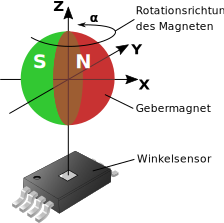
\includegraphics[width=0.35\linewidth]{chapters/images/2-Grundlagen/Klassischer_Anwendugsfall}
	\caption[Klassischer Anwendungsfall für die Drehwinkelerfassung]{Klassischer Anwendungsfall für die 
		Drehwinkelerfassung. Zeigt einen, um seine $Z$-Achse rotierenden, Gebermagneten und einen Winkelsensor in 
		zentrierter und orthogonaler Ausrichtung zur $Z$-Achse des Magneten. Idealerweise befinden sich Magnet und 
		Sensor, 
		ohne Verkippungen in $X$- oder $Y$-Richtung, parallel zueinander. Grafik entnommen und bearbeitet aus 
		\cite{Schuethe2020a}.}
	\label{fig:klassischeranwendugsfall}
\end{figure}


Durch die Phasenverschiebung der Sinus-Funktion stehen die Messwerte $V_{cos}(H_x,H_y)$ und $V_{sin}(H_x,H_y)$ 
vektoriell orthogonal zueinander. Bedingt durch die Orthogonalität der Messwerte $V_{cos}(H_x,H_y) \perp 
V_{sin}(H_x,H_y)$ und gleichförmige Kreisbewegung des Magneten um seine $Z$-Achse, beschreibt die Winkelmessung in 
polarer Darstellung eine konstante Kreisbahn. Diese besitzt einen konstanten Bahnradius $r$ und die Winkelstellung 
$\alpha$ des Gebermagneten \cite{Schuethe2019}.
\newline
Für eine beliebige Winkelmessung $\mathbf{A}$, die eine entsprechende Winkelstellung $\alpha$ des Gebermagneten 
abbildet $\mathbf{A}\mapsto\alpha$, ergibt sich somit folgender vektorieller Zusammenhang in \autoref{eq:vektorfeld} 
\cite{Schuethe2020}.


\begin{equation}\label{eq:vektorfeld}
\underbrace{\begin{pmatrix} H_x(\alpha) \\ H_y(\alpha) \end{pmatrix}}_{\textrm{Gebermagnetfeld}}\Rightarrow
\underbrace{
	\begin{pmatrix} V_{cos}(H_x,H_y) \\ V_{sin}(H_x,H_y) \end{pmatrix}}_{\textrm{Winkelsensormesswerte}}=
\underbrace{
	\begin{pmatrix} r\cdot\cos(\alpha) \\ r\cdot\sin(\alpha)\end{pmatrix}=
	\begin{pmatrix} a_x \\ a_y \end{pmatrix}}_{\textrm{Kreisdarstellung}}=
\underbrace{\mathbf{A}(\alpha) \vphantom{\begin{pmatrix}x\\y\end{pmatrix}}}_{\textrm{Winkelmessung}}
\end{equation}

Die so erhobenen Winkelmessung $\mathbf{A}$ nach \autoref{eq:vektorfeld}, bildet ein eindimensionales Vektorfeld mit 
$\{a_x,b_x\}\in\mathbb{R}$ ab. Wobei sich der Bahnradius $r$ für die Kreisdarstellung, aus dem Betrag der Messung 
$|\mathbf{A}|$, nach \autoref{eq:bahnradius} gewinnen lässt.


\begin{equation}\label{eq:bahnradius}
r = |\mathbf{A}| = \sqrt{\big(V_{cos}(H_x,H_y)\big)^2 + \big(V_{sin}(H_x,H_y)\big)^2} =\sqrt{a_x^2 + a_y^2}
\end{equation}


\clearpage


\begin{figure}[tph]
	\centering
	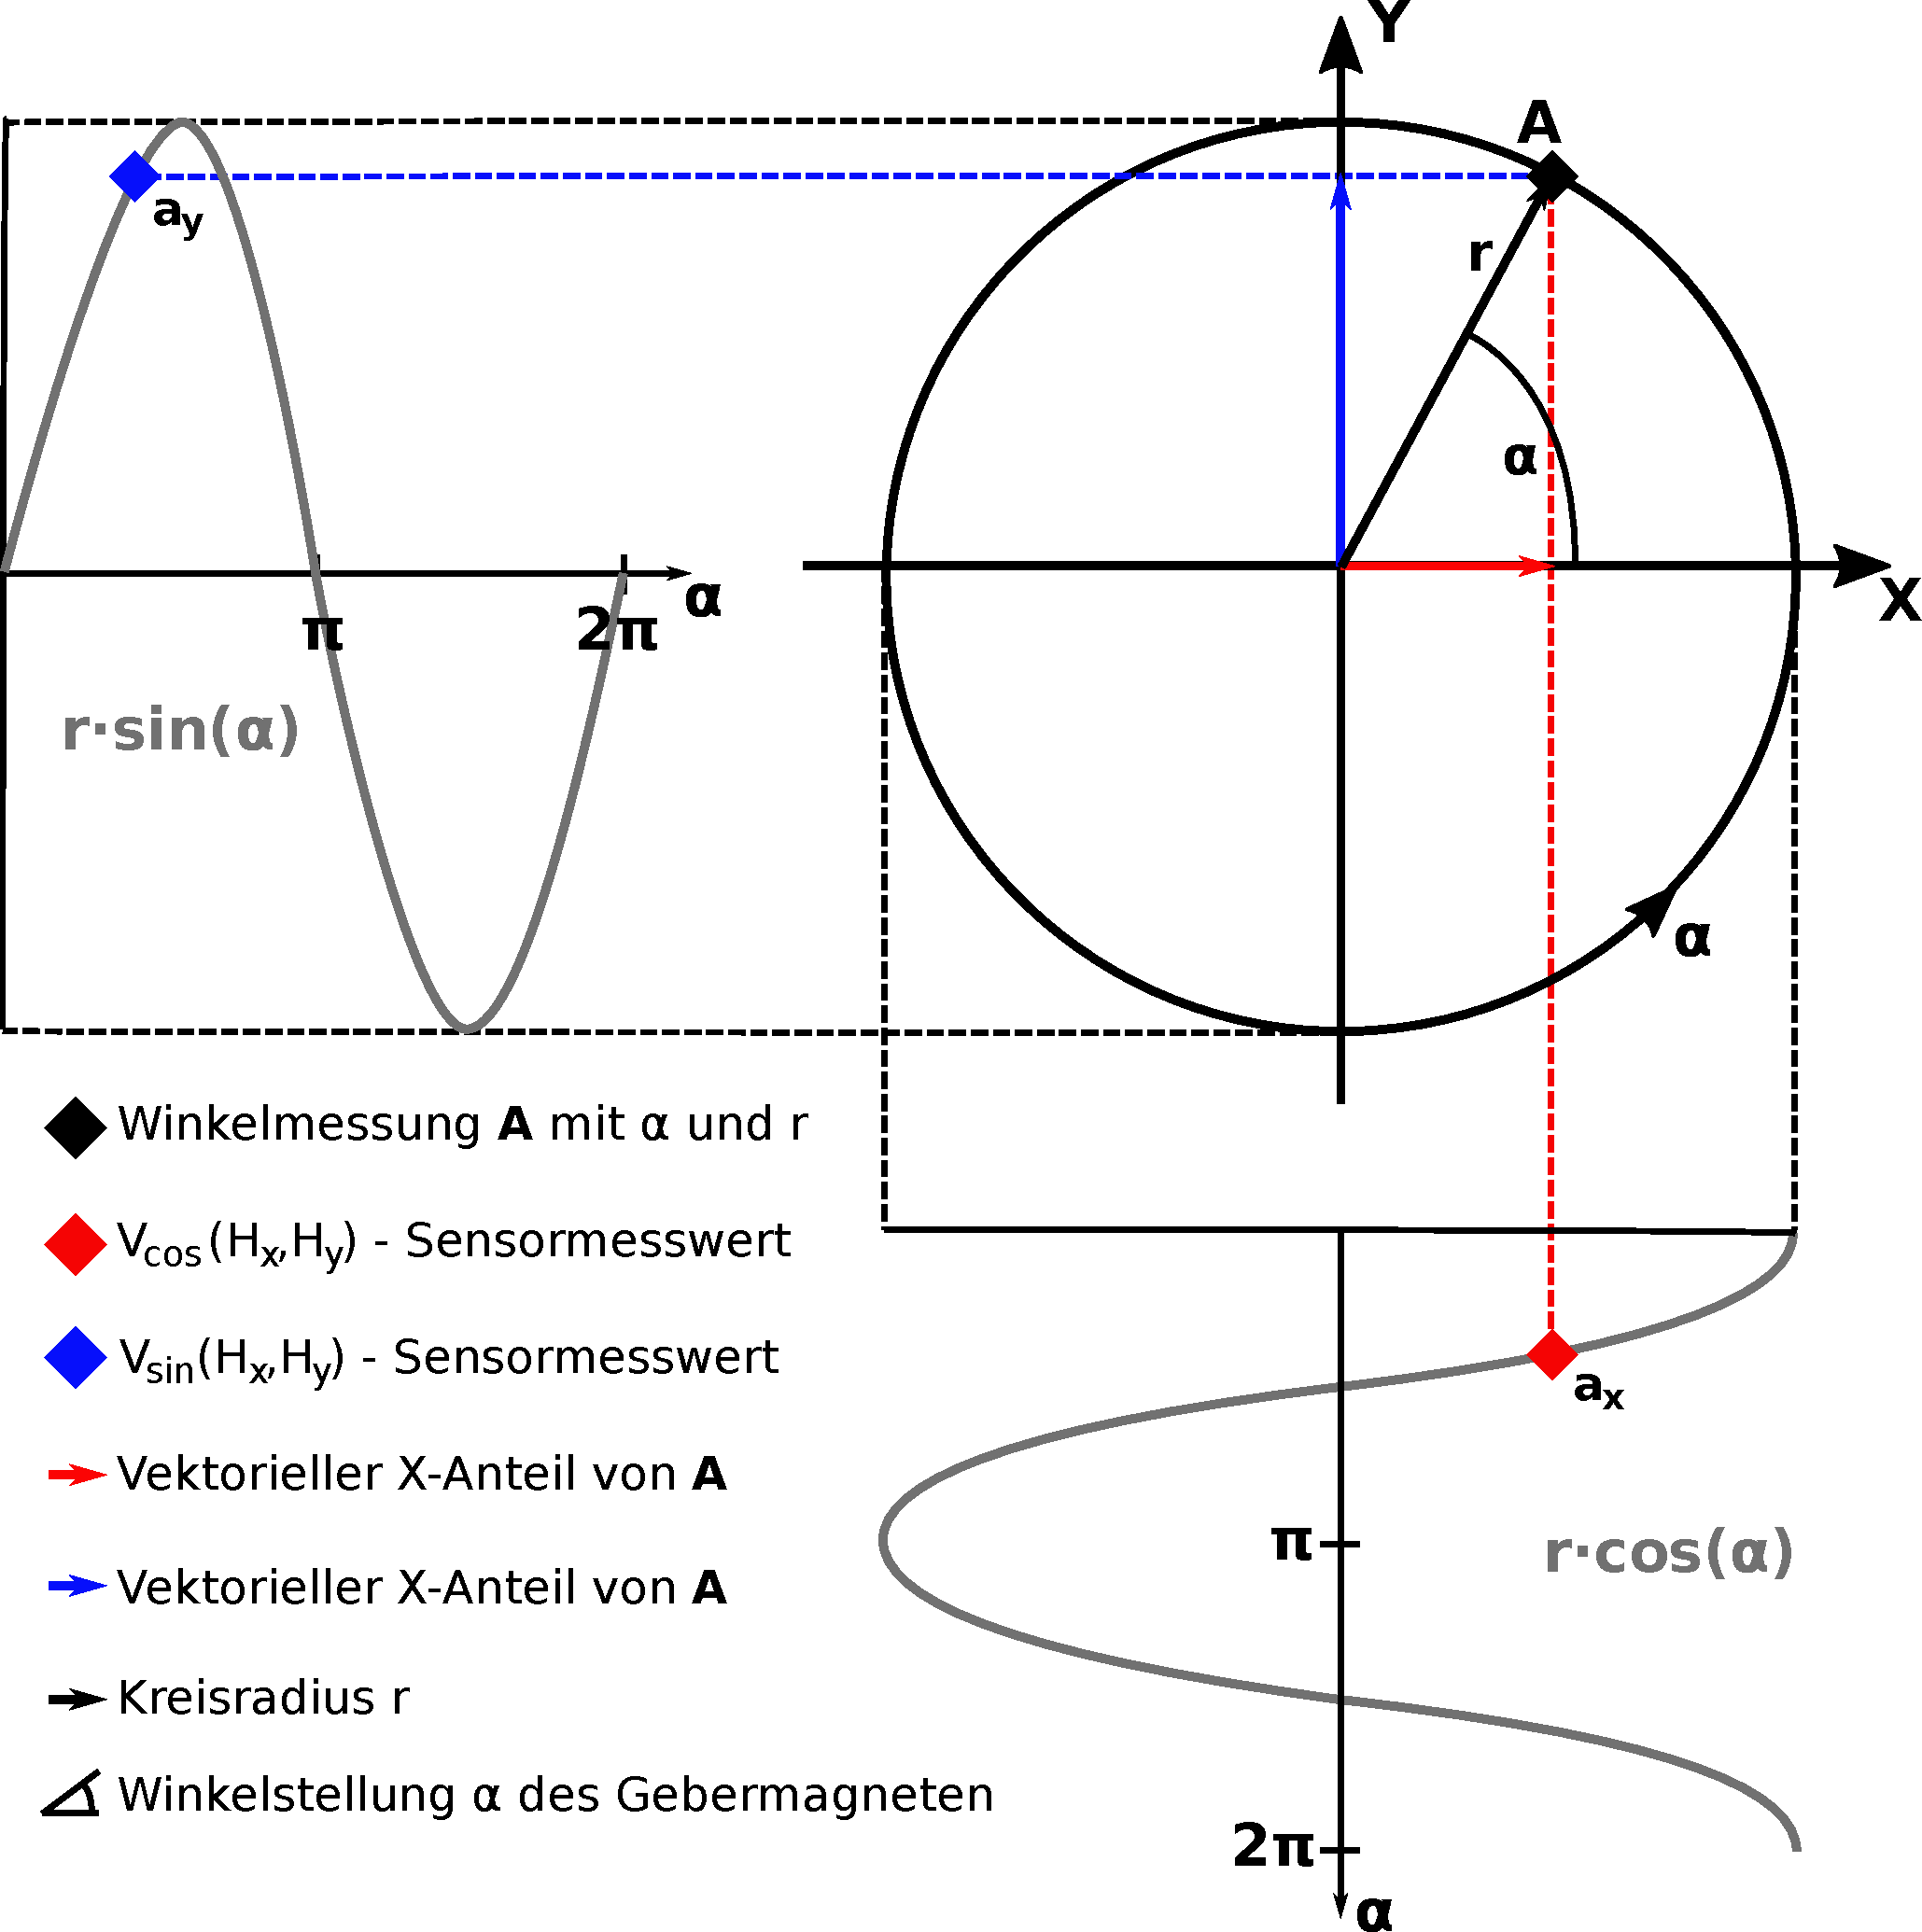
\includegraphics[width=0.7\linewidth]{chapters/images/2-Grundlagen/Kreisdarstellung_Winkelmessung}
	\caption[Kreisdarstellung der Winkelmessung]{Kreisdarstellung der Winkelmessung. Als Abbildung der
		Winkelmessung $\mathbf{A}\mapsto\alpha$ aus	\autoref{eq:vektorfeld}. Die Zusammensetzung der Messung erfolgt 
		durch, die vom Winkelsensor gemessenen, vektoriellen Anteile für die polare Darstellung der 
		Gebermagnetwinkelstellung.}
	\label{fig:kreisdarstellungwinkelmessung}
\end{figure}



% !TEX root = ../thesis.tex
% euclidic distance in norm notation
% @author Tobias Wulf
%

\section{Euklidischer Abstand in Normschreibweise}\label{sec:euklidischer-abstand}


Um adäquate Bezüge bzw. Abstände zwischen einzelnen Messwerten herzustellen ist ein Wechsel der Betrachtungsweise notwendig. Es erleichtert die Handhabung der Problemstellung Vektorbeträge als normierte Längen und Distanzen zu sehen. Betrachtet man die vektoriellen Zusammenhänge, der klassischen Anwendung aus \autoref{sec:kreisdarstellung-anwendung}, in Normschreibweise. Ergibt sich der Radius $r$ für eine Winkelstellung $\mathbf{A}\mapsto\alpha_1$ nach \autoref{eq:rinnorm}. Die einzelnen Vektorelemente sind entsprechend der Vektor-2-Norm \cite{vandeGeijn2014} zum Radius $r$ normiert.


\begin{equation}\label{eq:rinnorm}
r = |\mathbf{A}| =\sqrt{a_x^2 + a_y^2} = \sqrt{\sum_{i=1}^{n}|A_i|^2} = \|\mathbf{A}\|_2
\end{equation}


Es ist weithin von einer idealen Ausrichtung von Sensor und Gebermagnet wie in \autoref{fig:klassischeranwendungsfall} auszugehen. Somit bleibt der Kreisbahn Radius $r$ für eine zweite Winkelstellung mit $\mathbf{B}\mapsto\alpha_2$ konstant.


\begin{equation}
r = \|\mathbf{A}\|_2 = \|\mathbf{B}\|_2 = konst.
\end{equation}


Der direkte Abstand zwischen den beiden Winkelstellung $\mathbf{A}\mapsto\alpha_1$ und $\mathbf{B}\mapsto\alpha_2$ lässt sich geometrisch über den Satz des Pythagoras ermitteln. Dafür werden Abstandquadrate aus den Einzeldifferenzen der vektoriellen $X$-/ $Y$-Anteile gebildet. Das Resultierende Abstandsquadrat bildet mit seiner Kantenlänge dann den Winkelabstand zwischen beiden Winkelstellungen. \autoref{fig:kreisdarstellungwinkelabstand} veranschaulicht das Vorgehen.


\begin{align}\label{eq:deinnorm}
d_E\langle\mathbf{A},\mathbf{B}\rangle &= \sqrt{(a_x - b_x)^2 + (a_y - b_y)^2} \nonumber \\
&= \sqrt{\sum_{i=1}^{n}(A_i - B_i)^2} = \|\mathbf{A} - \mathbf{B}\|_2
\end{align}


\clearpage


Die Überführung in Normschreibweise des Abstandes ergibt nach \autoref{eq:deinnorm} eine Vektor-2-Differenznorm und ist allgemein als euklidischer Abstand bekannt. Analog dazu bildet sich das Quadrat nach \autoref{eq:de2innorm}.


\begin{equation}\label{eq:de2innorm}
d_E^2\langle\mathbf{A},\mathbf{B}\rangle = (a_x - b_x)^2 + (a_y - b_y)^2 = \|\mathbf{A} - \mathbf{B}\|_2^2
\end{equation}

\vspace{5mm}
\begin{figure}[bph]
	\centering
	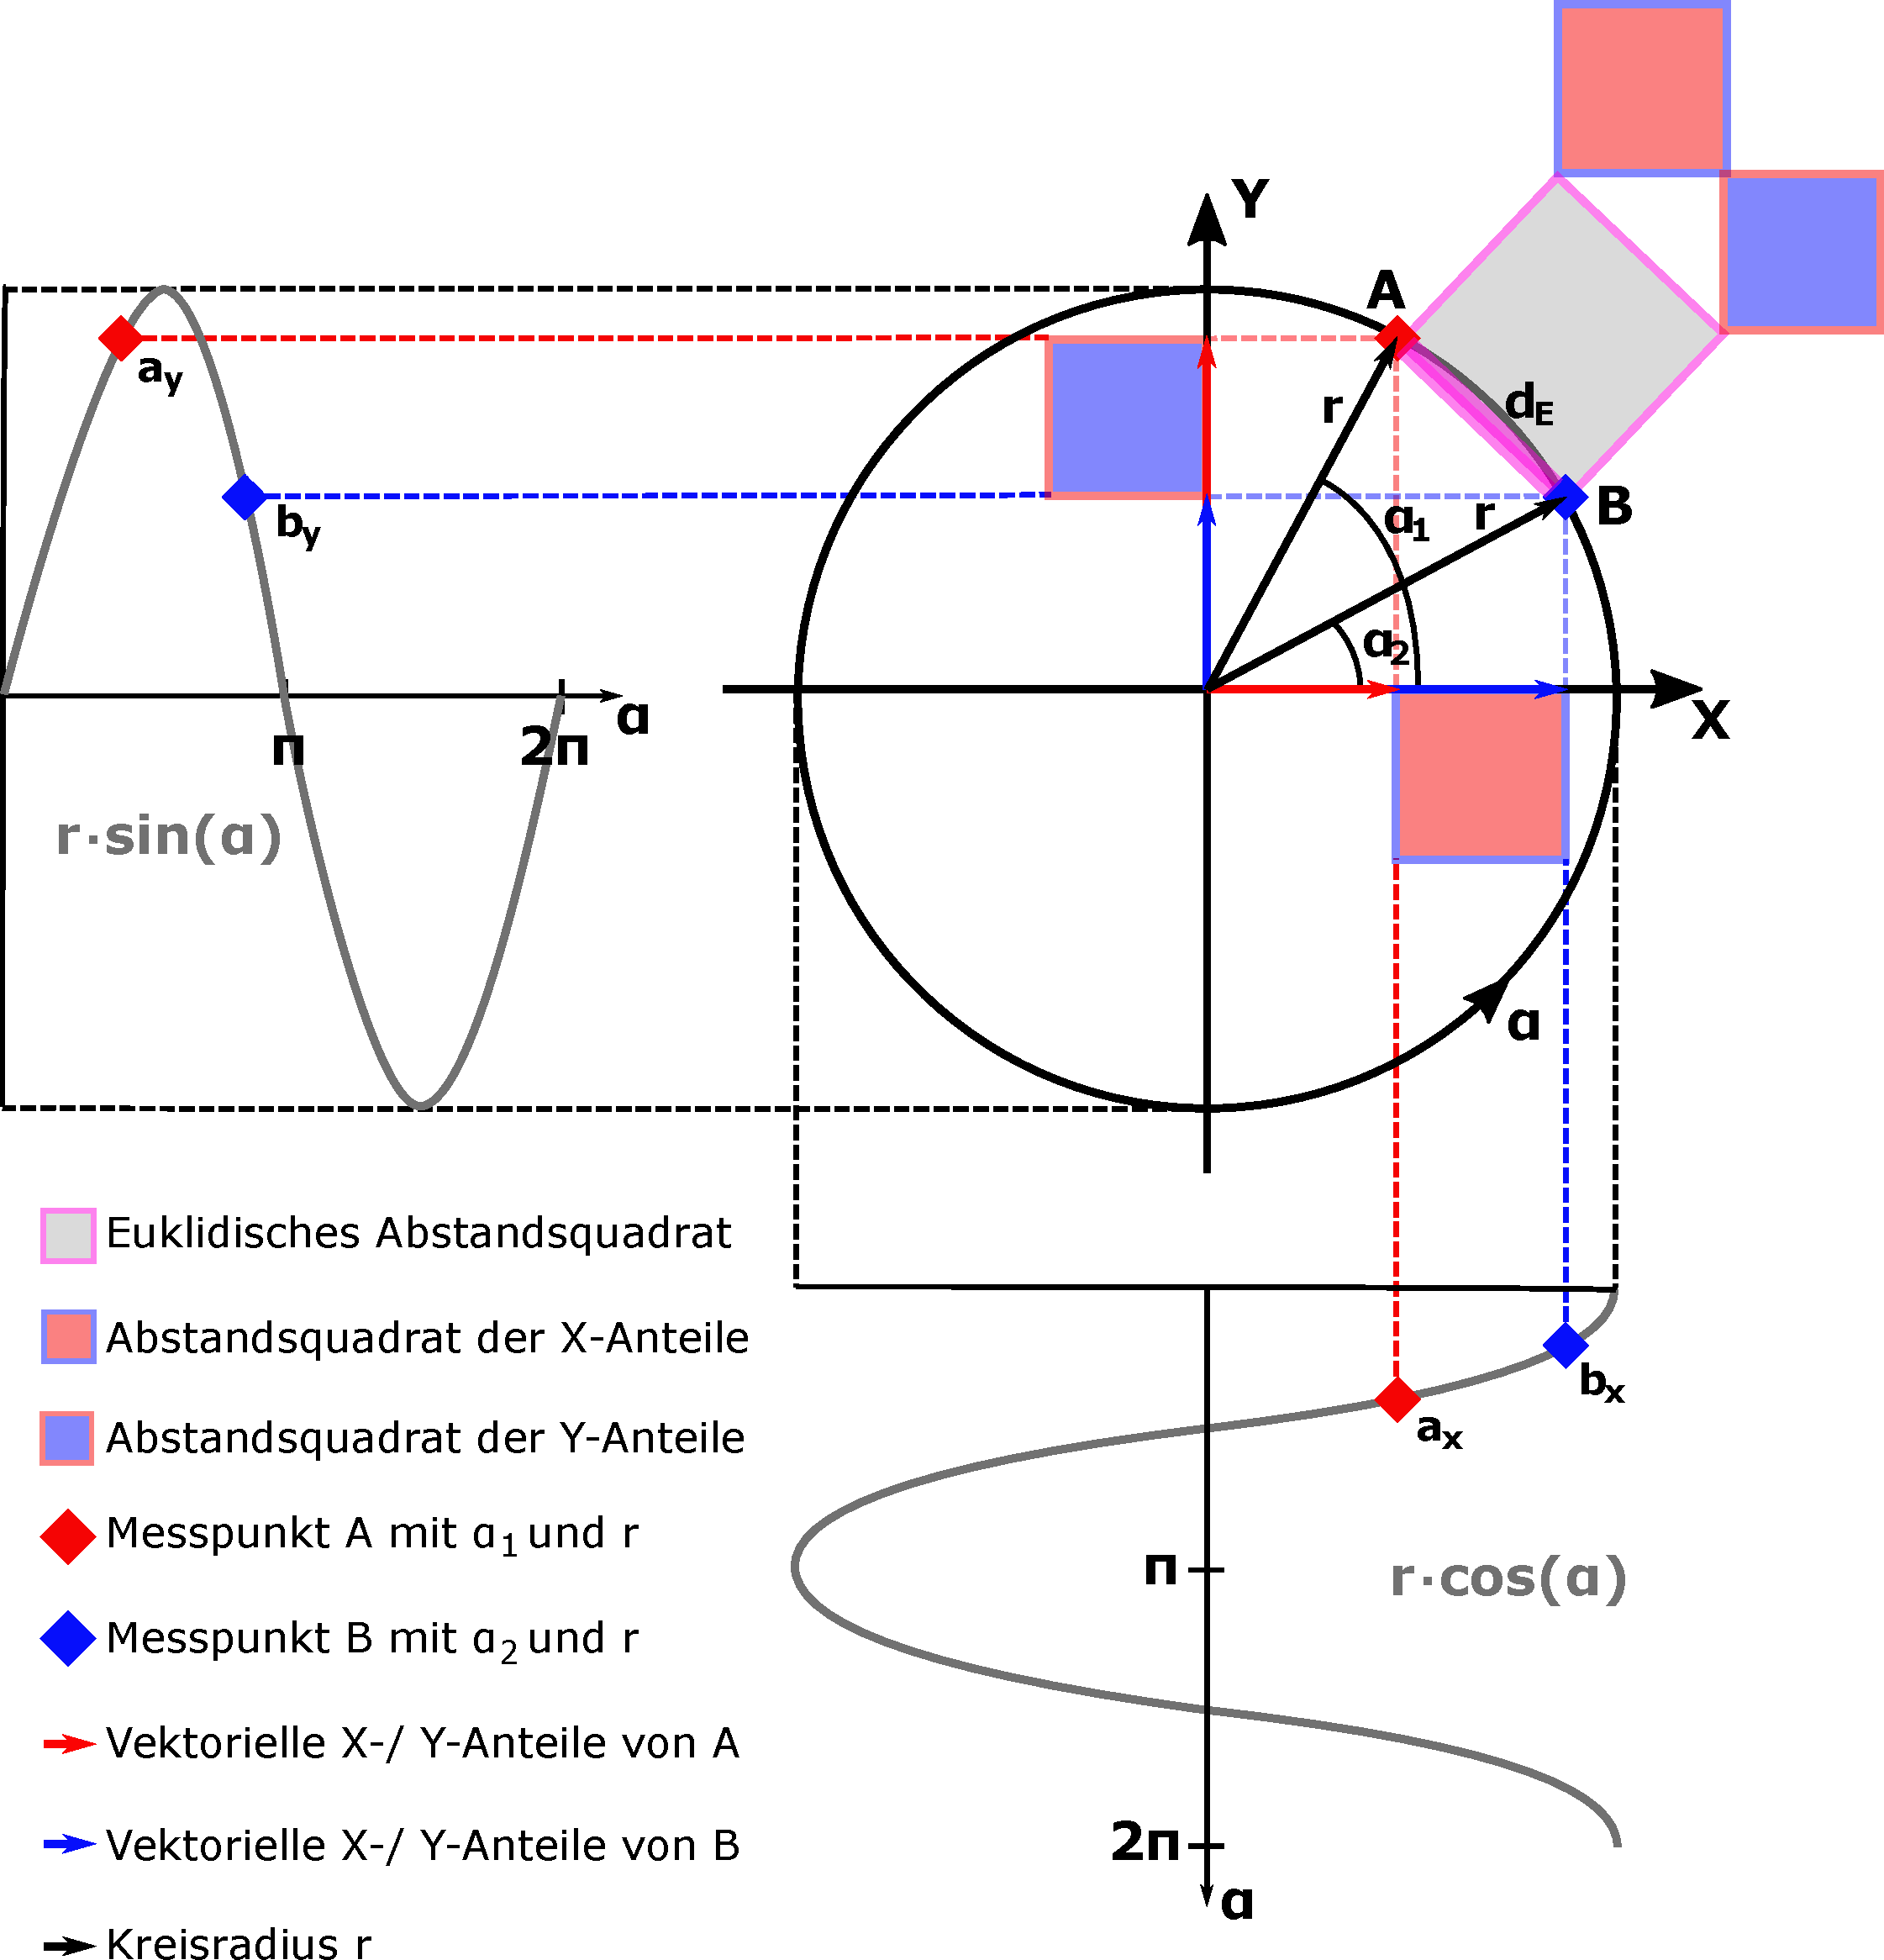
\includegraphics[width=0.7\linewidth]{chapters/images/2-Grundlagen/Kreisdarstellung_Winkelabstand}
	\caption[Allg. Kreisdarstellung des euklidischen Winkelabstands]{Allg. Kreisdarstellung des euklidischen 
		Winkelabstands. Die Kreisdarstellung zeigt den euklidischen Winkelabstand zweier Winkelmesspunkte $\mathbf{A}$ 
		und $\mathbf{B}$ mit gleichen Kreisradius $r$. Der euklidische Abstand, bzw. das Abstandsquadrat, zwischen den 
		Winkelposition $\mathbf{A}$ und $\mathbf{B}$ ist zerlegt in Abstandsquadratanteile. Die Abstandquadratanteile 
		ergeben sich aus der vektoriellen Zusammensetzung in $X$-/ $Y$-Anteile für die einzelnen Messpunkte 
		$\mathbf{A}$ und $\mathbf{B}$.}
	\label{fig:kreisdarstellungwinkelabstand}
\end{figure}


\clearpage


Für Vektor-2-Normen muss die Dreiecksungleichung aus \autoref{eq:v2ungleichung} \cite{Plum2012}\cite{vandeGeijn2014} gelten. Über die Ungleichung lassen sich Einzelnormen approximiert im Vergleich zu Differenznormen zwischen zwei Punkten $\mathbf{A}$ und $\mathbf{B}$ darstellen. Dieser Ansatz kann genutzt werden wenn die Bahnradius $r$ nicht mehr konstant ist und somit $\|\mathbf{A}\|_2 \ne \|\mathbf{B}\|_2$ ist. Der Ansatz begünstigt die Projektion von orthogonalen Systemen in höheren Normraum \cite{Plum2012} und stellt somit die Grundlage für eine Adaptierung auf ein Sensor-Array dar.


\begin{gather}\label{eq:v2ungleichung}
\big| \|\mathbf{A}\|_2 - \|\mathbf{B}\|_2 \big| \le
	\|\mathbf{A} \pm \mathbf{B}\|_2 \le \big| \|\mathbf{A}\|_2 + \|\mathbf{B}\|_2 \big| \nonumber \\
\Updownarrow \\
\big(\|\mathbf{A}\|_2 - \|\mathbf{B}\|_2\big)^2 \le \|\mathbf{A} \pm \mathbf{B}\|_2^2 \le
	\big(\|\mathbf{A}\|_2 + \|\mathbf{B}\|_2\big)^2 \nonumber
\end{gather}


% !TEX root = ../thesis.tex
% magnetic sensors and angular detection
% @author Tobias Wulf
%

\section{Magnetische Sensoren und Drehwinkelerfassung}\label{sec:magnetische-sensoren}


Magnetische Sensoren besitzen eine lange Tradition in der Automobilindustrie. Sie eignen sich besonders durch die berührungslose Erfassung von mechanischen Bewegungen und die kontaktlose Strommessung für den Einsatz in der Fahrzeugtechnik. Es existieren verschiedene Sensoren, die durch unterschiedliche magnetoresistive Effekte realisiert sind. Dabei bildet sich das Grundprinzip, durch anlegen eines äußeren Magnetfeldes und eine resultierende Änderung des elektrischen Widerstandes eines Materials \cite{Tille2020}.


\vspace{5mm}
\begin{figure}[tbph]
	\centering
	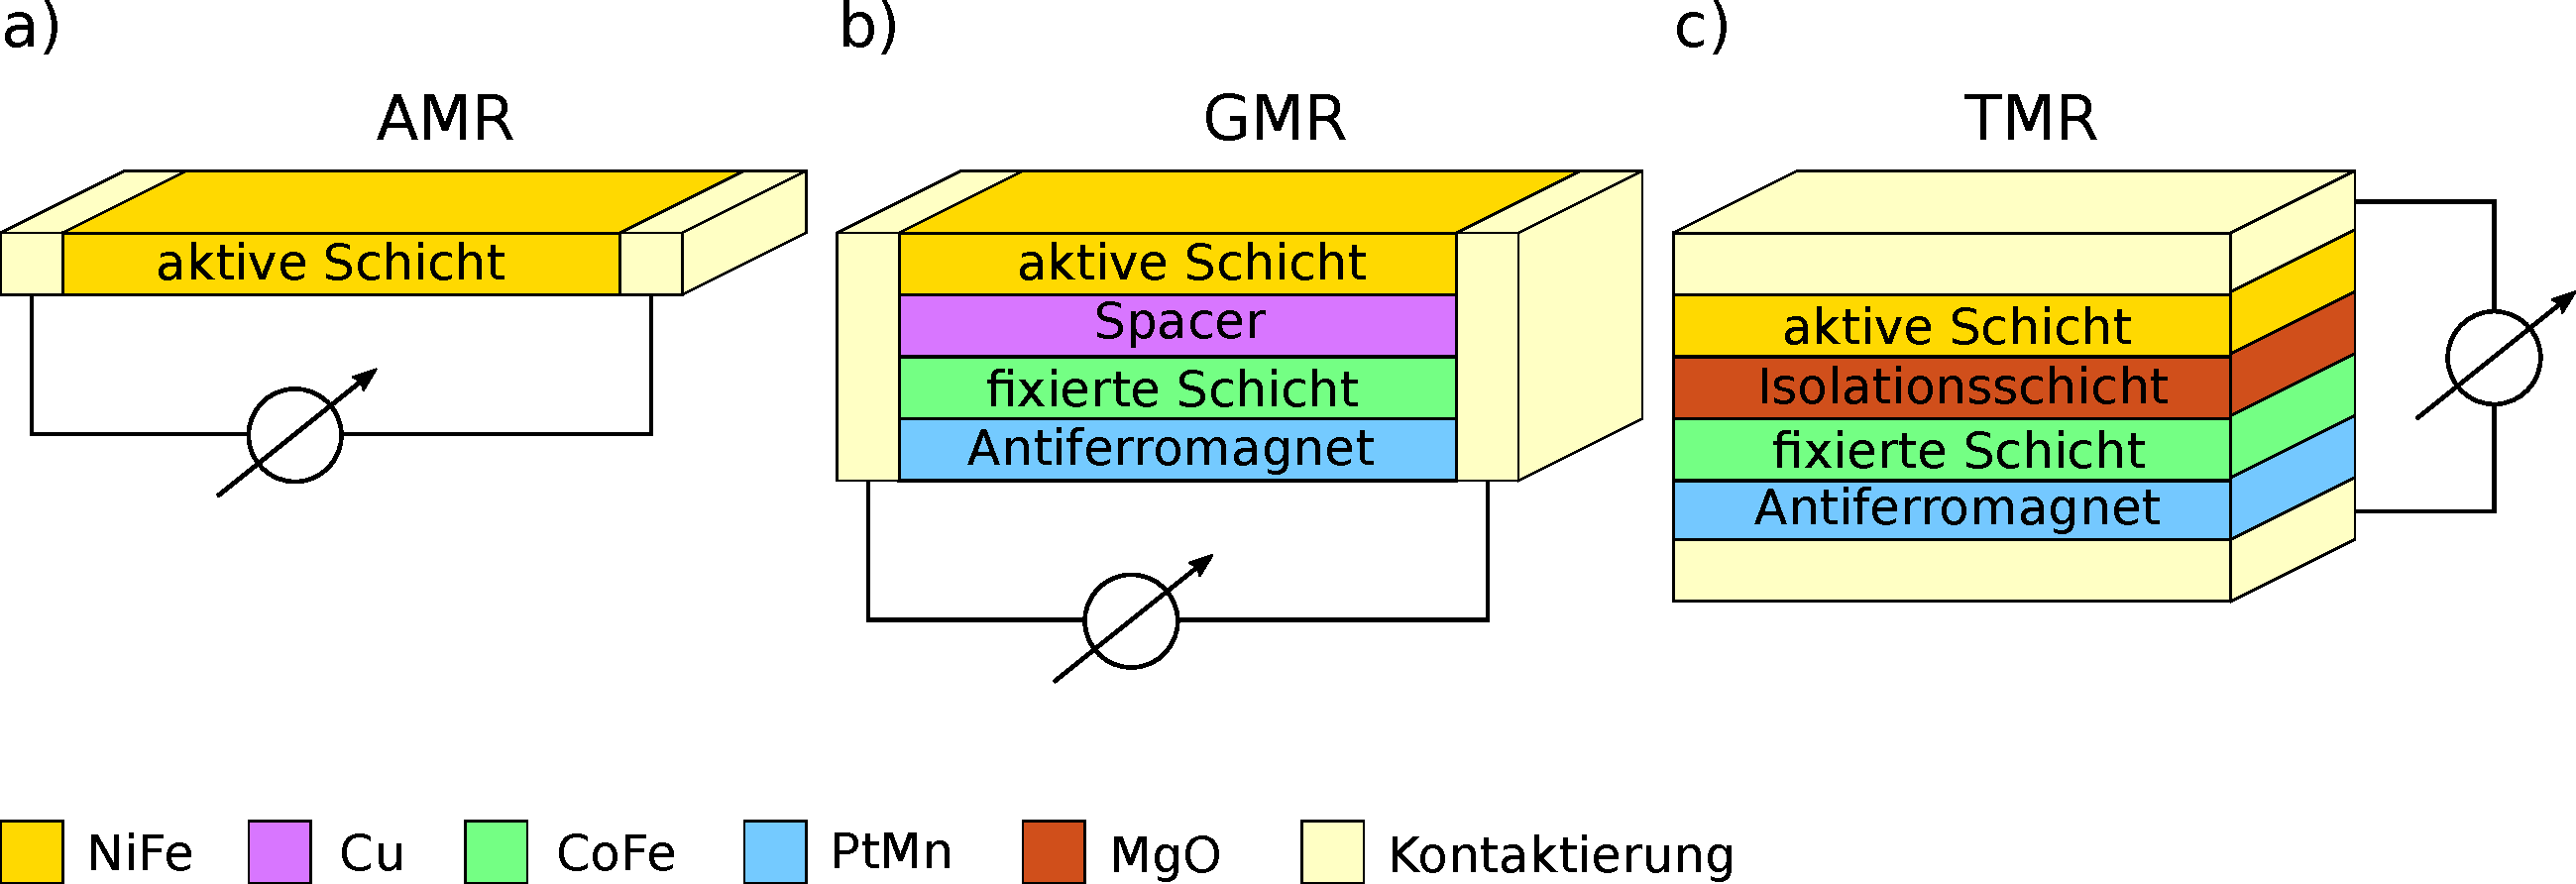
\includegraphics[width=\linewidth]{chapters/images/2-Grundlagen/MR_Schichtmodelle}
	\caption[Schichtmodelle dreier magnetoresistive Effekte]{Schichtmodelle dreier magnetoresistive Effekte. a) 
		\gls{gl:amr}, schwache Widerstandsänderung. b) \gls{gl:gmr} stärkere Widerstandsänderung. c) \gls{gl:tmr} stärkste 
		Widerstandsänderung. Grafik entnommen aus \cite{Lemme2016}.}
	\label{fig:mrschichtmodelle}
\end{figure}


\clearpage


\paragraph{AMR-Effekt}\label{par:AMR}$~$\\


In der Mitte des 19. Jahrhunderts entdeckte der britische Physiker William Thomson den anisotropen magnetoresistiven Effekt (AMR). Der \gls{gl:amr} basiert auf einer von Strom- und Magnetisierungsrichtung abhängigen Streuung von Elektronen in einer einzelnen aktiven Schicht, Teil a) der \autoref{fig:mrschichtmodelle}. Diese Schicht besteht in der Praxis oftmals aus einer Nickel-Eisen-Legierung. Die typische Variation der relativen Widerstandsänderung $\Delta R/R$ liegt im Bereich von $2\%$ bis $3\%$ \cite{Tille2020}. Für eine eindeutig Winkelmessung werden zwei Wheatstone'sche Brücken aus dem Schichtmaterial aufgebaut. Die Stromdurchflussrichtung ist horizontal. Bedingt durch den \gls{gl:amr} ist eine Periodizität von $\SI{180}{\degree}$ abgedeckt \cite{Lemme2016}\cite{Tille2020}. Ein mittels \gls{gl:amr} entwickelter Sensor für die Drehwinkelerfassung, besitzt daher zwei um $\SI{45}{\degree}$ verdrehte Wheatstone-Brücken. Durch die schwache Widerstandsänderung des Materials ist eine nachgeschaltet Verstärkerschaltung notwendig \cite{NXPSemiconductors2014}.


\paragraph{GMR-Effekt}\label{par:GMR}$~$\\


Der riesiger magnetoresistive Effekt, engl. \gls{ac:gmr},  ist 1988 von Grünberg und Fert entdeckt worden. Beide erhielten dafür 2007 den Nobelpreis für Physik, da unter Ausnutzung des \gls{gl:gmr}s sich die Speicherkapazität von Computerfestplatten stark erhöhen lies \cite{Lemme2016}. Das Minimalprinzip für einen solchen Sensor bildet sich aus zwei magnetischen Dünnschichten, die durch eine nicht magnetische Schicht (z.B. Kupfer) voneinander getrennt sind. Dabei folgt die Magnetisierung der aktiven Schicht (z.B. Nickel-Eisen) einem von außen angelegten Magnetfeld, während die Magnetisierung der zweiten Schicht (z.B. Kobalt-Eisen) durch eine darunter liegende antiferromagnetische Schicht (z.B. Platin-Mangan) fixiert ist. Die Stromdurchflussrichtung bleibt wie beim AMR horizontal \cite{Lemme2016}\cite{Tille2020}. Die relativen Widerstandsänderung $\Delta R/R$ ist abhängig von der relativen Ausrichtung der Magnetisierungen in beiden magnetischen Schichten und liegt für einfache Schichtsystem, wie in Teil b) der \autoref{fig:mrschichtmodelle} gezeigt, bei etwa $10\%$. Die Herstellung eines GMR-Sensors ist deutlich aufwendiger, als es beim \gls{gl:amr} der Fall ist. So können aber in Multilagen mit vielfacher Wiederholung der magnetischen Schichten bis zu
$80\%$ $\Delta R/R$ erreicht werden \cite{Tille2020}. Mit der GMR Technologie aufgebaute Drehwinkelsensoren haben eine Periodizität von 360° und besitzen zwei um $\SI{90}{\degree}$ verdrehte Wheatstone-Brücken und ebenfalls nachgeschaltete Verstärkereinheiten \cite{infineon2018}.


\paragraph{TMR-Effekt}\label{par:TMR}$~$\\


Im Jahr 1975 ist der tunnel-magnetoresistive Effekt (TMR) durch M. Jullière entdeckt worden. Im einfachsten Fall, wie Teil c) \autoref{fig:mrschichtmodelle} zeigt, tritt der Effekt bei Schichtsystemen auf, die durch eine isolierende Schicht (z.B. Magnesiumoxid) getrennt sind \cite{Lemme2016}. Die Stromdurchflussrichtung ist im Gegensatz zum AMR und GMR vertikal zu den Schichten. Die relativen Widerstandsänderung $\Delta R/R$ erfolgt in Abhängigkeit zur relativen Ausrichtung der Magnetisierungen beider magnetischen Schichten, die an der Isolationsschicht angrenzen.
\newline
Wie beim GMR folgt die aktive Schicht einem äußeren Magnetfeld, ebenso ist die zweite Schicht durch eine antiferromagnetische Schicht fixiert  \cite{Tille2020}. Der zugrunde liegende Effekt ist aber physikalisch ein gänzlich anderer. Hier ``tunnelt'' der Stromfluss durch die Isolationsschicht. Das ist ein quantenmechanischer Effekt und kann mit Ansätzen der ``normalen'' Physik nicht mehr erklärt werden. Zurückzuführen ist der Effekt auf die Spin-Polarisation der einzelnen Elektroden eines magnetischen Tunnel-Kontaktes \cite{Tille2020}.
\newline
In praktischen Ausführungen bei Raumtemperatur liegen heute relative Widerstandsänderungen $\Delta R/R$ im Bereich von $30\%$ bis zu $200\%$ und sind somit deutlich höher als beim GMR \cite{Tille2020}. Unter Laborbedingungen konnten bei sehr tiefen Temperaturen mittlerweile Widerstandsänderungen bis zu $1000\%$ erreicht werden \cite{Lemme2016}.
\newline
Praxistaugliche Ausführungen von TMR-Sensoren stehen erst seit einigen Jahren zur Verfügung. Die Herstellung eines Sensors erfordert einen enormen apparativen Aufwand und Produktionsanlagen mit entsprechenden Fertigkeiten mussten erst entwickelt werden. Der Aufwand ist mit Vorteilen gegenüber dem AMR- und GMR-Sensor entlohnt worden.
Somit besitzt ein TMR-Sensorelement einen viel höheren Widerstand bei gleicher Abmessung. AMR/ GMR Technologien müssen im Vergleich flächenhungrige Strukturen realisieren. Aufgrund der vergleichsweise kleinen Flächen und einer äußerst geringeren Stromaufnahme ist ein engmaschiger Aufbau von Array-Strukturen möglich \cite{Lemme2016}. TMR-Flächen sind typischer Weise $< \SI{2}{\micro\metre}$ im  Radius. Die hohe Widerstandsänderung generiert entsprechend hohe Signalamplituden in der Magnetfelderfassung, daher kann eine nachgeschaltete Verstärkung entfallen. Es ist eine Periodizität von $\SI{360}{\degree}$ abgedeckt. Ein TMR-Sensor für die Drehwinkelerfassung besteht aus zwei um $\SI{90}{\degree}$ verdrehte Wheatstone-Brücken \cite{TDK2016}.


\clearpage

\paragraph{Wheatstone-Brücke}\label{par:wheatstone-bruecke}$~$\\


Ein einzelnes TMR-Element bzw. Widerstand kann bereits als eigenständiger magnetischer Sensor betrachtet werden. Allerdings können Temperatureinflüsse den Widerstand mitunter variieren lassen. Um den Temperatureinfluss entgegenzuwirken, sind daher \gls{gl:wheatstonebruecken} genutzt. Die einzelnen Widerstände der Brücke sind dabei so angeordnet, dass sie einen gemeinsamen Temperaturkoeffizienten besitzen und entsprechend miteinander gleichmäßig Schwanken \cite{Tille2020}. Über die Differenzmessung an den Brückenmittelabgriffen wird somit der Temperatureinfluss weitestgehend unterdrückt \cite{TDK2016}\cite{Tille2020}. \autoref{fig:tmrdrehwinkelapplikation} zeigt den schematischen Brückenaufbau für einen TMR-Sensor. Bei gleichförmiger Rotation eines Anregungsmagnetfeld wird durch die $\SI{90}{\degree}$ Verdrehung beider Brücken zueinander erreicht, dass diese benötigte Cosinus- und Sinus-Funktion, mit entsprechender Phasenverschiebung um $\SI{90}{\degree}$, für den Anwendungsfall in \autoref{sec:kreisdarstellung-anwendug} ausgeben \cite{TDK2016}. 


\vspace{5mm}
\begin{figure}[tbph]
	\centering
	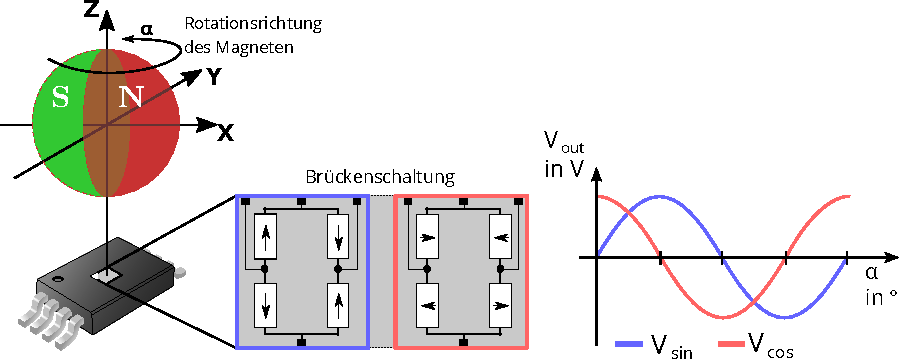
\includegraphics[width=\linewidth]{chapters/images/2-Grundlagen/TMR_Drehwinkelapplikation}
	\caption[TMR Drehwinkelapplikation]{TMR Drehwinkelapplikation. Schematisch gezeigt für eine volle Rotation des 
		Gebermagneten um $\SI{360}{\degree}$. Zu sehen sind die um $\SI{90}{\degree}$ verdrehten Wheatstone-Brücken des 
		Sensors. Die Brücken bilden, bei rotierenden Gebermagnetfeld, eine Sinus- und Cosinus-Funktion nach. Die Pfeile in 
		den einzelnen Widerständen weisen auf ihre magnetische Ausrichtung hin. Grafik entnommen und bearbeitet aus 
		\cite{Schuethe2020a}.}
	\label{fig:tmrdrehwinkelapplikation}
\end{figure}

% !TEX root = ../thesis.tex
% senor characterization
% @author Tobias Wulf
%

\section{Kennfeldmethode zur Charakterisierung von Sensoren}\label{sec:kennfeldmethode-zur-charakterisierung}


Die physikalisch-mathematische Beschreibung von magnetischen Sensormodellen, für eine simulative Nutzung, ist nicht trivial. Jede in \autoref{sec:magnetische-sensoren} zusammengefasste Sensortechnologie birgt bestimmte verhaltensbezogene Eigenschaften in sich. So müssen technologiebasierte Abhängigkeiten in Linearität und Sättigungsverhalten in komplexen mathematischen Gleichungen beschrieben sein. Wobei bestimmte Parameter der Modelle experimentell bestimmt werden müssen \cite{Schuethe2019}. Das stellt einen erheblichen Arbeitsaufwand dar. Der \gls{gl:ags} ist es gelungen diesen Aufwand durch Messmethodik zu umgehen. So ist die \gls{gl:kennfeldmethode} zur Charakterisierung von magnetoresistiven Sensoren entwickelt worden. Das ziel der Messmethode ist es repräsentative Datensätze zu generieren, die physikalische Charakteristiken eines Sensors in sich vereinigen und sein Verhalten zur weiteren Nutzung zugänglich machen.
\newline
Im Labor der \gls{gl:ags} sind automatisierte Messstände für Sensoren verschiedenster Couleur eingerichtet. Je nach Sensortechnologie und Applikation können diese mit unterschiedlichen Messmitteln bestückt werden. So ist es möglich die richtige Stimulanz für die jeweilige Sensorapplikation zu erzeugen. Für das Ausmessen von Winkelsensoren ist ein \gls{gl:kreuzspulenmessstand} zur Anwendung gekommen \cite{Schuethe2019}\cite{Schuethe2020}. Der Messstand eignet sich besonders gut dazu rotierende Magnetfelder zu erzeugen. Was einer idealen Stimulanz für Winkelsensoren entspricht. Das Magnetfeld wird dabei durch ein speziell abgestimmtes \gls{gl:kreuzspulensystem} erzeugt. Die dafür eingespeisten Spulenströme sind dabei direkt proportional zum erzeugten Magnetfeld. Das Anregungsfeld kann somit über Spulenfaktoren zurückgerechnet werden \cite{Schuethe2020}.
\newline
\autoref{fig:magnetfeldstimuluskennfeldmethode} zeigt das verwendete Anregungsfeld zur Charakterisierung. Stimuliert wird in $X$- und $Y$-Richtung, der räumlichen Sensorebene. So verwendet die $H_x$-Feldgenerierung ein dreicksmodulierter Cosinus-Strom. Die $H_y$-Feldgenerierung nutzt ein, mit gleicher Frequenz, dreicksmodulierten Sinus-Strom. Es entstehen dabei steigende und fallende Modulationsflanken bzw. Messverläufe. Es ergeben sich in polarer Darstellung Trajektorien mit wachsender und schrumpfende Amplituden, die durch Rotation einen nach Außen (steigend) bzw. Innen (fallend) gerichteten Verlauf besitzen \cite{Schuethe2019}. Es werden die Spulenströme und Spannungsausgaben des Sensors aufgezeichnet.
\newline
In einem weiteren Evaluierungsschritt sind Stimuli und Sensorsignale programmatisch zu indizieren, um eine gegenseitig Referenzierung zu ermöglichen. Sodass resultierend zweidimensionale \gls{gl:kennfeldpaar}e, bestehend aus je ein \gls{gl:kennfeld} für entsprechende Winkelsensor-Wheatstone-Brücke, als Charakterisierungsergebnis zur Verfügung stehen \cite{Schuethe2019}.


\clearpage


\begin{figure}[tbph]
	\centering
	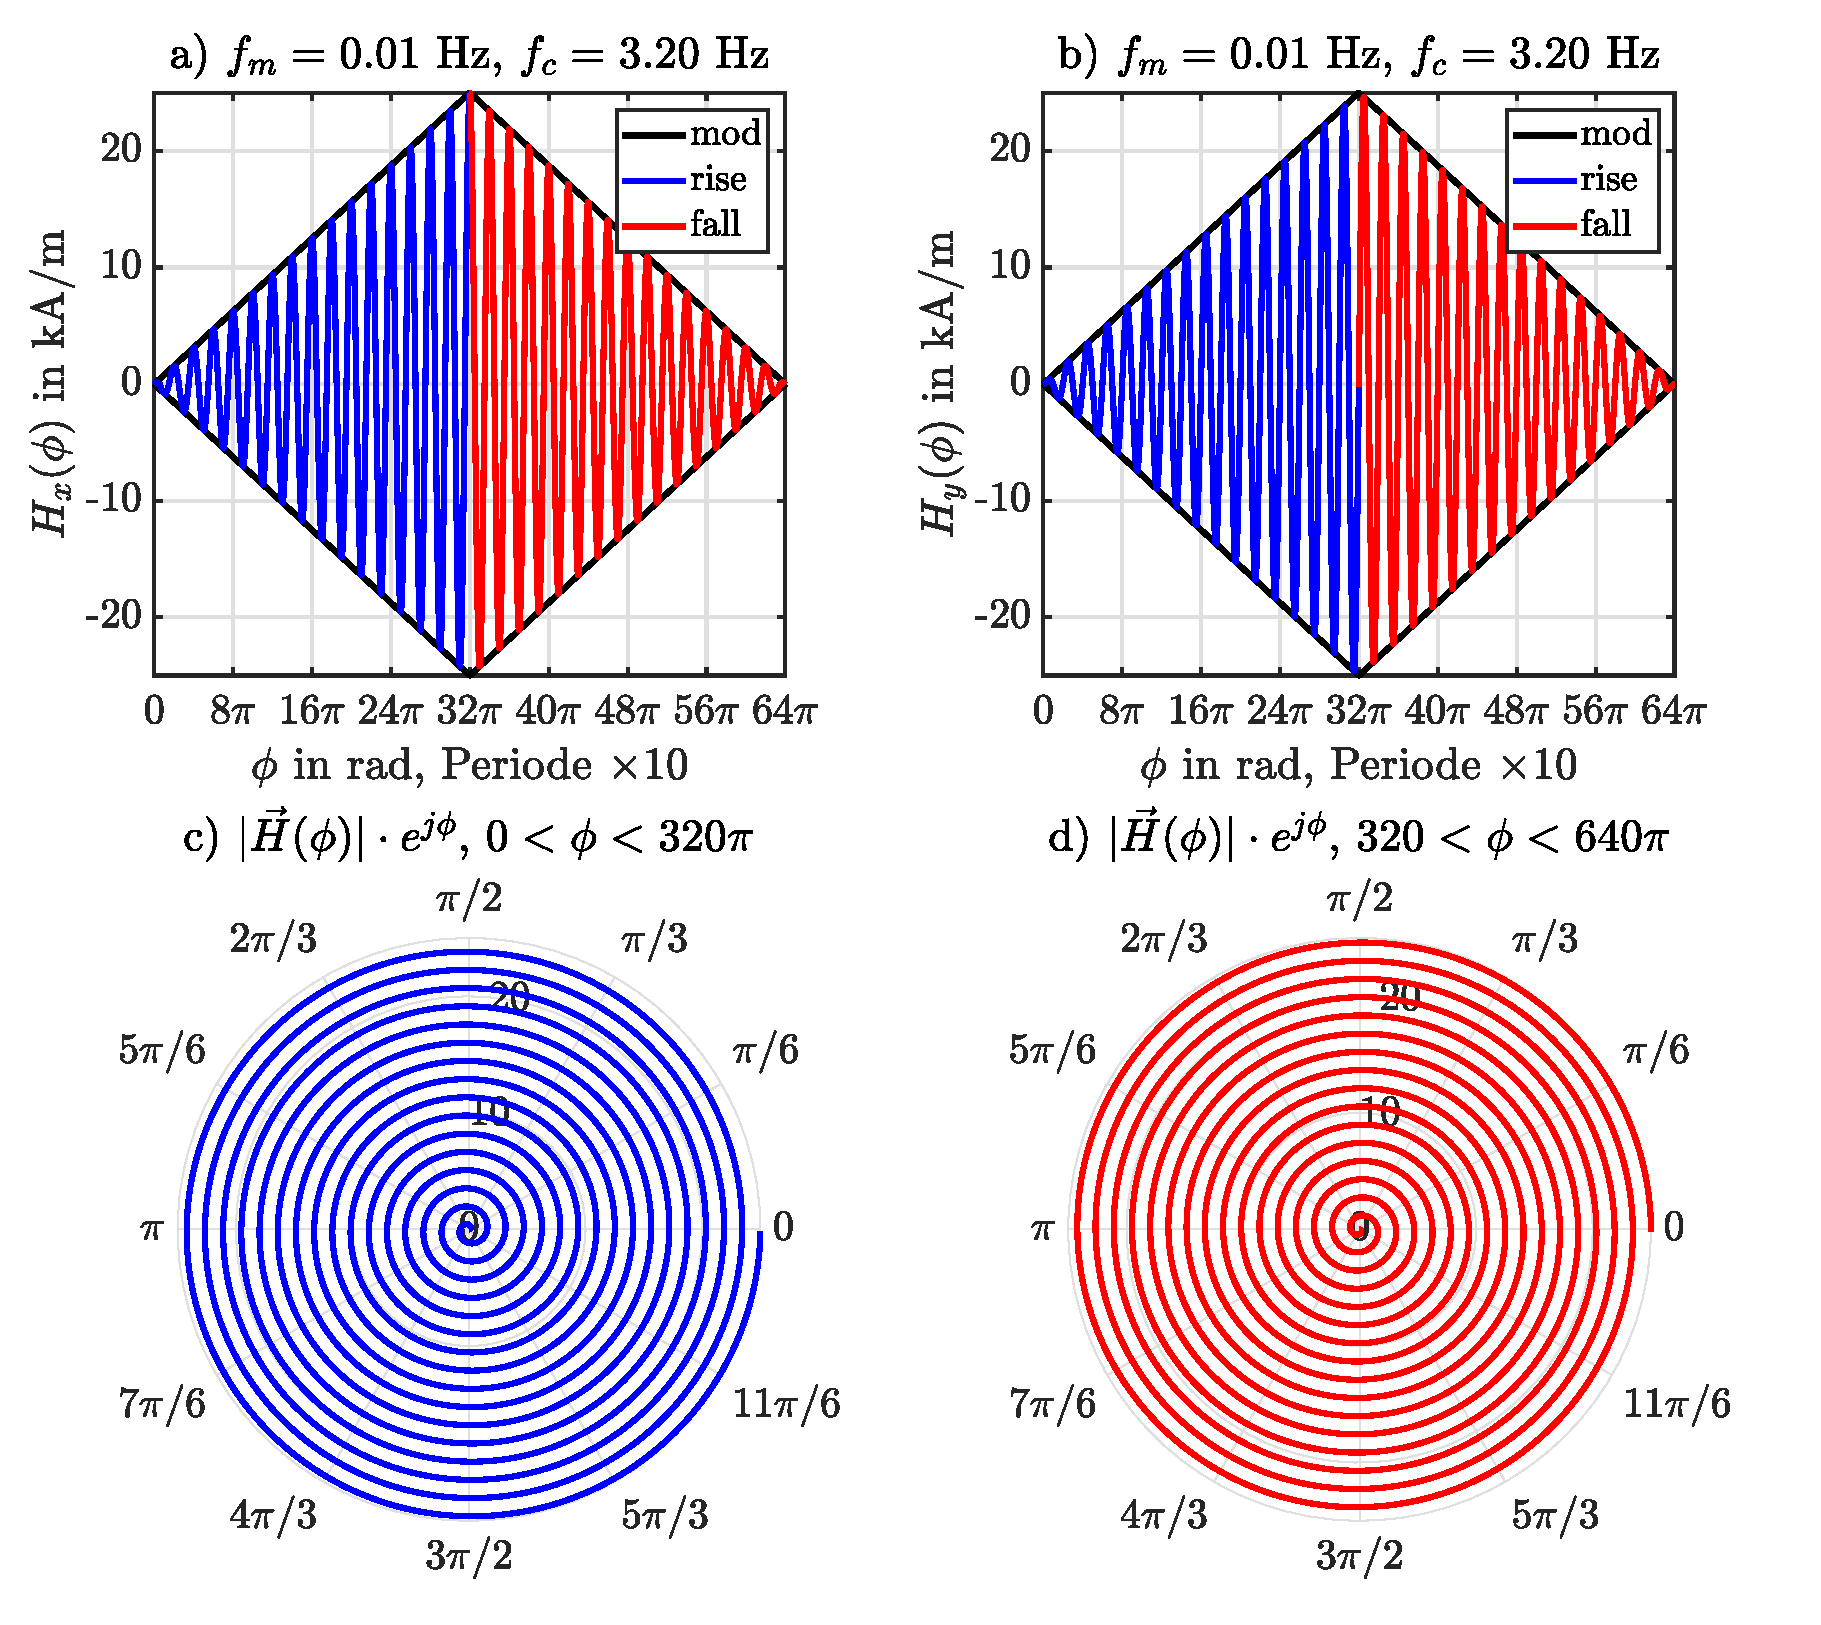
\includegraphics[width=\linewidth]{chapters/images/2-Grundlagen/Magnetfeldstimulus_Kennfeldmethode}
	\caption[Magnetfeldstimulus zur Erzeugung von Sensorkennfeldern]{Magnetfeldstimulus zur Erzeugung von 
		Sensorkennfeldern. Es sind die Bestandteile des magnetischen Sensorstimuli dargestellt, die zum Ausmessen des 
		Sensorkennfeldes in $H_x$- und $H_y$-Richtung verwendet worden sind. Es ist das Prinzip des Verfahrens 
		dargestellt. In a) und b) ist die Dreiecksmodulation des magnetischen Anregungsfeldes abgebildet. Für a) die 
		$H_x$-Feldanregung mit Cosinus-Trägerwelle und für b) die $H_y$-Feldanregung mit Sinus-Trägerwelle. Es sind für 
		beide Anregungsrichtungen niedrige Frequenzen gewählt um ein quasi-statisches Anregungsmagnetfeld zu erzeugen. 
		Es ergeben sich für die Betragsamplitude des Stimulus, in polarer Darstellung c) und d), konzentrische 
		Trajektorien. Diese verlaufen von Innen nach Außen für die steigende Flanke der Amplitudenmodulation c) und von 
		Außen nach Innen für die fallende Flanke d). Die Dreieckmodulationsfrequenz liegt bei $f_m = \SI{0.1}{\hertz}$ 
		und einer Trägerwellenfrequenz $f_c = \SI{3.2}{\hertz}$. Grafik nachempfunden aus \cite{Schuethe2019}.}
	\label{fig:magnetfeldstimuluskennfeldmethode}
\end{figure}


\clearpage


Im \autoref{ch:tdk-datensatz} ist der Kennfelddatensatz eines TMR-Sensors \cite{TDK2016} gezeigt. Der Datensatz dient, als Arbeitsgrundlage für die Sensor-Array-Simulation und ist von der \gls{gl:ags} zur Verfügung gestellt worden. Zur Simulation sind die Kennfelder aus \autoref{fig:TDKuebertragungskennlinien} zu verwenden, a) für die Erzeugung der Cosinus-Funktion und b) für die Sinus-Funktion. Beide Kennfelder zeichnen sich besonders durch ihren linearen Arbeitsbereich zwischen $\pm\SI{8,5}{\kilo\ampere\per\metre}$ aus. Der Arbeitsbereich ist für beide Kennfelder nahezu identisch, zu sehen in c) und als Kreis in a) und b) markiert. 


\vspace{5mm}
\begin{figure}[tbph]
	\centering
	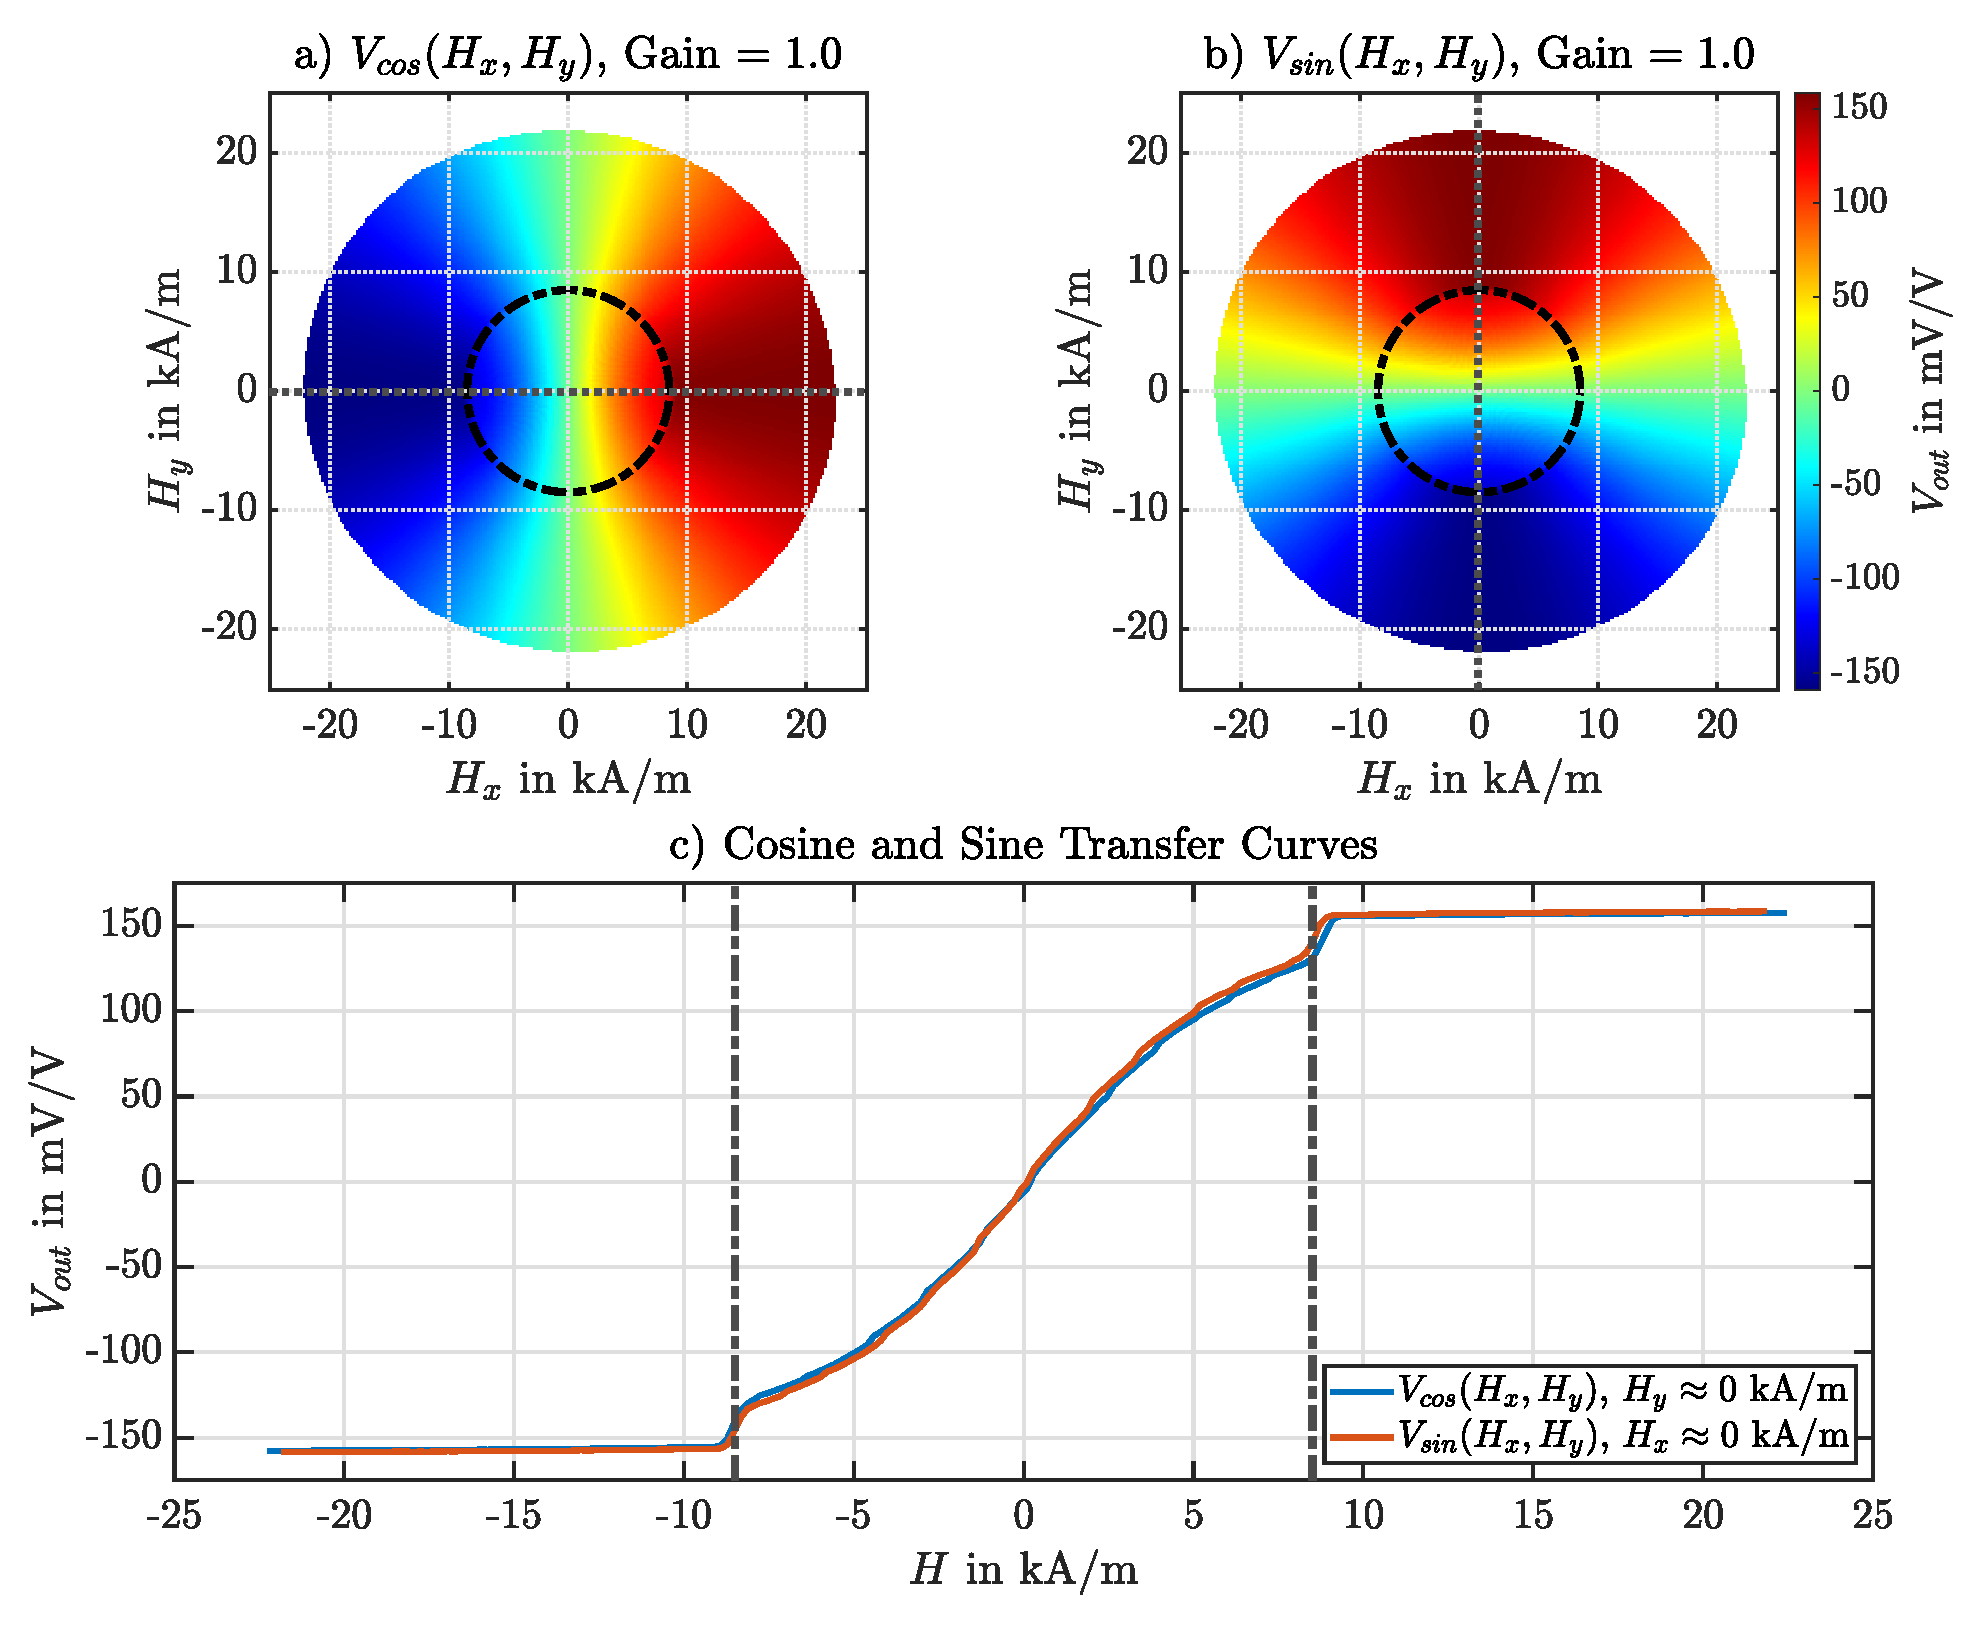
\includegraphics[width=.95\linewidth]{chapters/images/2-Grundlagen/TDK_Uebertragungskennlinien}
	\caption[TDK TAS2141-AAAB Übertragungskennlinie]{TDK TAS2141-AAAB Übertragungskennlinie. Es sind wieder die 
		Kennfelder aus der steigenden Amplitudenmodulation in a) und b). In c) sind die Übertragungskennlinien für den 
		Sensor gezeigt mit Kennzeichnung für den Betrieb auf dem linearen Plateau des Kennfeldes bei 
		$\SI{8.5}{\kilo\ampere\per\metre}$. Ebenfalls zu sehen in a) und b) durch die sich ergebene Kreisbahn mit einem 
		Radius des aufgelegten Intervalls aus c). Grafik nachempfunden aus \cite{Schuethe2019}.}
	\label{fig:TDKuebertragungskennlinien}
\end{figure}


\clearpage


\vspace{5mm}
\begin{figure}[tph]
	\centering
	\includegraphics[width=.7\linewidth]{chapters/images/2-Grundlagen/Approximierter_Kugelmagnet}
	\caption[Approximierter Kugelmagnet]{Approximierter Kugelmagnet. Die Approximation des Kugelmagneten erfolgt 
		über Dipol-Feldgleichung in Näherung des Kugelmagnetfernfeldes. Das Magnetfeld ist auf 
		$\SI{200}{\kilo\ampere\per\metre}$ bei einem Abstand von $\SI{1}{\milli\metre}$ zur Kugelmagnetoberfläche 
		normiert. Der Radius des Kugelmagneten beträgt $\SI{2}{\milli\metre}$.}
	\label{fig:dipolemagnet}
\end{figure}


Auf den TMR-Sensor-Kennfeldern basierende Simulationen, sollten daher so parametriert sein, dass sie innerhalb des markierten Bereiches stattfinden. Zur Generierung von Spannungsausgaben in einer Sensorsimulation, sind für korrespondiere Anregungsfeldstärken entsprechende Referenzwerte aus den Kennfeldern zu entnehmen. Die  Referenzwerte sind normiert und nach \autoref{eq:vout-tdk} in Spannungsausgaben der Wheatstone-Brückenschaltungen umzurechnen. Ein geeignetes Verfahren für die Entnahme von Referenzwerten bietet hier, die in Matlab implementierte $2D$-Interpolation. Diese kann so parametriert werden, dass sie nach dem Nearest-Neighbor-Verfahren für beliebige Feldstärkeneingaben den nächstgelegen Referenzwert ausgibt. Wichtig sind hierbei eine gute magnetische Stimulanz, die den Arbeitsbereich des Kennfeldes trifft. Als Beispiel für eine passende Anregung soll hier, der in \autoref{fig:dipolemagnet} approximierte, Kugelmagnet dienen. Das Magnetfeld ist so normiert das eine Betragsfeldstärke von $\SI{200}{\kilo\ampere\per\metre}$ bei $\SI{1}{mm}$ Abstand zur Magnetenoberfläche anliegt. Die angelegte Skala zeigt, dass ein Sensor mit seinen Kennfeldern aus \autoref{fig:TDKuebertragungskennlinien}, einen Abstand in $Z$-Richtung größer als $\SI{6}{\milli\metre}$ einhalten sollte, um den Arbeitsbereich des Kennfeldes zu treffen. Weitere Beschreibungen und Erläuterungen zur Simulation und Dimensionierung der magnetischen Feldanregung finden sich im \autoref{sec:sensor-array-simulation-dipol-feldgleichung}.




% !TEX root = ../thesis.tex
% sensor-array prinziple
% @author Tobias Wulf
%

\section{Prinzip des Sensor-Arrays}\label{sec:prinzip-des-sensor-arrays}


Ein \gls{gl:sensor-array} stellt in seiner Funktionsweise ein Array aus einzelnen Winkelsensoren dar. Jeder einzelne Winkelsensor des Arrays bildet somit einen \gls{gl:sensor-pixel}. Die einzelnen Sensor-Pixel besitzen im Simulationsbetrieb das selbe Verhalten, das basierend auf den TMR-Senor \cite{TDK2016}, aus Kennfeldern (\autoref{ch:tdk-datensatz}) entnommen wird. Resultierende Messwerte der einzelnen Sensor-Pixel sind positionsabhängig von ihrer Lage im Sensor-Array\cite{Schuethe2019}. Die Sensor-Pixel-Anordnung erfolgt quadratisch mit gleichen Abständen zu einander. Das Gesamtsystem ist somit eine Adaption des klassischen Anwendungsfall aus \autoref{fig:klassischeranwendungsfall} für multiple Winkelsensoren \cite{Mehm2019}\cite{Schuethe2019}. So ergibt sich der Anwendungsfall für das Sensor-Array nach \autoref{fig:sensor-array-prinzip}.
\newline
Das Gesamtsystem aus Gebermagnet und Sensor-Array behält seinen Koordinatenursprung in der Gebermagnetmitte. Das Sensor-Array ist zentriert und lotrecht zur $Z$-Achse des Magneten auszurichten \cite{Schuethe2019}. Sodass ein konstantes Flächenniveau in $Z$ eingehalten wird. Bedingt durch die aufgespannte Array-Fläche, sind die einzelnen Sensor-Pixel nicht mehr ideal unter dem Magneten ausgerichtet \cite{Schuethe2020b}. Es ist somit davon auszugehen, dass die Kreisbahnen der einzelnen Pixel verzerrt sind. Wobei sich die Bahnbeschreibungen, der Pixel mit dem geringsten $X$-/ $Y$-Versatz, einem idealen Kreisverlauf annähern müssen. Physikalische Kleinstabstände zwischen den Sensorbrücken eines Sensor-Pixels sind vernachlässigt. Im Simulationsbetrieb ist die Annahme getroffen, dass die Brückenabstände innerhalb eines Sensor-Pixel vernachlässigbar klein sind.


\clearpage


\begin{figure}[tph]
	\centering
	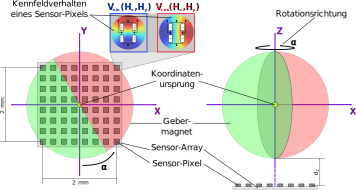
\includegraphics[width=.9\linewidth]{chapters/images/2-Grundlagen/Sensor-Array-Prinzip}
	\caption[Geometrischer Aufbau und Ausrichtung des Sensor-Arrays]{Geometrischer Aufbau und Ausrichtung des Sensor-Arrays. Quadratische Anordnung von Sensor-Pixeln zu einem $8 \times 8$ Sensor-Array. Alle Pixel sind gleich verteilt auf der Array-Fläche. Sensor-Pixel-Verhalten ist aus Kennfeldern entnommen und ortsabhängig von Pixel-Position im Koordinatensystem. Array-Kantenlängen sind mittig von Eck-Pixel zu Eck-Pixel bestimmt. Ebenfalls der $Z$-Abstand zur Magnetoberfläche. Abstände innerhalb der Pixel sind vernachlässigt. Das Array ist zentriert in der $Z$-Achse ausgerichtet. Ideal lotrecht zur Nord-Süd-Ausrichtung des Magneten. Koordinatenursprung des Gesamtsystem liegt in der Gebermagnetmitte. Gebermagnet ist ein Kugelmagnet, der um seine $Z$-Achse rotiert. Grafik nachempfunden und bearbeitet aus \cite{Schuethe2020b}.}
	\label{fig:sensor-array-prinzip}
\end{figure}


Gemäß der geometrischen Vorgaben, konstantem Flächenniveau in $Z$ und der Wahl des Koordinatenursprungs, fächert sich ein Koordinaten-Meshgrid für $N_{Pixel} \times N_{Pixel}$ für $i,j \in \{1 \ldots N_{Pixel} \}$ Sensor-Pixel auf. Dabei ist von einer, im Mittelpunkt des Sensor-Array festgelegten, Grundposition $\vec{p}$ des Sensor-Arrays nach \autoref{eq:arraymeshgrid} vorzugehen. 


\begin{alignat}{3}\label{eq:arraymeshgrid}
	&\vec{p} = \begin{pmatrix}p_x \\ p_y \\ p_z\end{pmatrix} \qquad && A_{Array} = a_{Array}^2 \qquad 					  && x_{i,j} = p_x - \frac{a_{Array}}{2} + j \cdot d_{Pixel} \nonumber\\
	& 																&& d_{Pixel} = \frac{a_{Array}}{N_{Pixel} - 1} \qquad && y_{i,j} = p_y + \frac{a_{Array}}{2} - i \cdot d_{Pixel} \\
	& 																&& 													  && z_{i,j} = p_z - r_{mag} = konst.\nonumber
\end{alignat}


Die  $Z$-Koordinate entspricht dem $Z$-Abstand zum Magneten mit $d_z = p_z$. Das Sensor-Array ist über diesen Vektor in Koordinatensystem zu verschieben. Der Koordinatenursprung bleibt im Magneten. Das Meshgrid fächert sich für die $i-te$ Reihe und die $j-te$ Spalte des Sensor-Arrays auf. Somit gibt jedes Sensor-Pixel, entsprechend seiner Zuordnung im Array, Spannungsausgaben wie ein einzelnes Sensor-IC aus. Es stehen dadurch nicht mehr Skalare bzw. ein Vektor als Winkelmesswert zur Verfügung, sondern Array-Daten für korrespondierende Cosinus- und Sinus-Vektorfelder \cite{Mehm2019}\cite{Schuethe2020}. \autoref{fig:sensor-array-daten} zeigt den dimensionalen Zuwachs. 


\vspace{5mm}
\begin{figure}[tph]
	\centering
	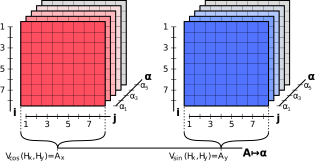
\includegraphics[width=0.9\linewidth]{chapters/images/2-Grundlagen/Sensor-Array-Daten}
	\caption[Resultierende Sensor-Array-Daten]{Resultierende Sensor-Array-Daten. Zwei Matrizen, je eine für alle Cosinus-Brückenausgaben und Sinus-Brückenausgaben. Die $i-ten$ und $j-ten$ Matrixelemente bilden eine Vektor entsprechend des klassischen Anwendungsbeispiels. Jeweils ein Matrix-Paar für die $n-te$ Winkelstellung $\alpha$.}
	\label{fig:sensor-array-daten}
\end{figure}


Bedingt durch den Zuwachs an Daten und ihre Anordnung, benötigt es eine modifizierte Abstandsfunktion \cite{Schuethe2020b}\cite{Schuethe2020} im Vergleich zur \autoref{eq:de2innorm}. Als erstes braucht es skalare Repräsentanten der Matrizen. Diese sind durch eine zutreffende Matrix-Norm zu bilden. Matrizen können als lange Vektoren betrachtet werden, daher bietet sich die Rechenvorschrift für $j-te$ Spalten nach \autoref{eq:fnorm} an. Diese Norm ist als Frobenius-Norm bezeichnet.


\begin{equation}\label{eq:fnorm}
\|\mathbf{A_x}\|_F= \sqrt{\sum_{j=1}^{n}\|A_{xj}\|_2^2} = \sqrt{\mathbf{A_x}\mathbf{A_x}^T}
\end{equation}


\clearpage


Angewandt auf beide Vektormatrizen für Cosinus- und Sinus-Anteile, ergibt sich eine normierte Kreisbahn nach \autoref{eq:rinfnorm}. Der Radius ist durch Versatz der einzelnen Sensor-Pixel nicht konstant und muss je nach Position des Sensor-Arrays eine weniger oder stärkere Ellipsenform beschreiben \cite{Schuethe2019}. Das ergibt sich durch Überlagerung der Sinoiden nach Frobenius-Norm. Der Versatz jedes einzelnen Sensor-Pixel wirkt dabei wie eine Dämpfung auf die Ausgangsspannungen der Sensor-Pixel. So zeigt sich ein Versatz in $X$-Richtung in einer Dämpfung der Cosinus-Funktion und entsprechender Versatz in $Y$-Richtung mit einer Dämpfung der Sinus-Funktion \cite{Schuethe2019}.


\begin{equation}\label{eq:rinfnorm}
	\|r\|_F = \big|\|\mathbf{A}\|_F\big| = \sqrt{\|\mathbf{A_x}\|_F^2 + \|\mathbf{A_y}\|_F^2}
\end{equation}


Durch simples einsetzen der normierten Messwertmatrizen in die euklidische Abstandsquadratfunktion \autoref{eq:de2innorm}, folgt ein approximiertes Abstandsergebnis nach \autoref{eq:fnorminde2}. Über die Dreiecksungleichung erhält man die genau Lösung und Projektion in den höheren Normraum \cite{Plum2012}\cite{vandeGeijn2014} und somit die modifizierte Abstandsfunktion nach Frobenius-Norm \cite{Schuethe2020}\cite{Schuethe2020b} in \autoref{eq:df2}. Es sind gemachte Beschreibungen aus \autoref{sec:euklidischer-abstand}, für zwei Winkelstellungen $\mathbf{A}$ und $\mathbf{B}$, entsprechend der Array-Datenformate angepasst.


\begin{align}
\label{eq:fnorminde2}
d_E^2\langle\mathbf{A},\mathbf{B}\rangle &= \big(\|\mathbf{A_x}\|_F - \|\mathbf{B_x}\|_F\big)^2 + \big(\|\mathbf{A_y}\|_F - \|\mathbf{B_y}\|_F\big)^2 \\
&\le \nonumber \\
\label{eq:df2}
d_F^2\langle\mathbf{A},\mathbf{B}\rangle &= \|\mathbf{A_x} - \mathbf{B_x}\|_F^2 + \|\mathbf{A_y} - \mathbf{B_y}\|_F^2 = \|\mathbf{A} - \mathbf{B}\|_F^2
\end{align}


\clearpage


% !TEX root = ../thesis.tex
% sensor array simulation with dipole field equation
% @author Tobias Wulf
%

\section{Sensor-Array-Simulation über die Dipol-Feldgleichung}\label{sec:sensor-array-simulation-dipol-feldgleichung}


Die Sensor-Array-Simulation nutzt einen Kugelmagneten als Stimulanz \cite{Schuethe2019}. Es ist die Anwendungsbeschreibung aus \autoref{fig:sensor-array-prinzip} gewählt. Der Vorteil darin liegt, dass ein Kugelmagnetfernfeld mittels der Feldgleichung für einen magnetischen Dipol approximiert werden kann \cite{Pape2017}. Das innere Magnetfeld des Kugelmagneten ist dabei zu vernachlässigen. Der Radius des Kugelmagneten $r_{mag}$ ist als Offset für den räumlichen Abstand zum Magneten zu verwenden. Weitere physikalische Effekte wie magnetische Remanenz werden vernachlässigt.



\begin{figure}[ph]
	\centering
	\includegraphics[width=0.7\linewidth]{chapters/images/2-Grundlagen/Dipol-Feldgleichung}
	\caption[Simulation der Dipol-Feldgleichung]{Simulation der Dipol-Feldgleichung. Als veranschaulichendes Beispiel ist ein Magnetfeld über die Dipol-Feldgleichung simuliert. Der Dipol bildet den Koordinatenursprung bei $\vec{r} = (0,0,0)^T$. In Relation zum Dipol ist ein Meshgrid der einzelnen Sensor-Pixel-Positionen $\vec{r}$ unterhalb des Dipols gelegt. Abhängig vom magnetischen Moment $\vec{m}$ des Dipols, wird an jeder Meshgrid-Position $\vec{r}$ die Dipol-Feldgleichung gelöst und punktuell die magnetische Feldstärke $\vec{H}$ berechnet. Das magnetische Moment $\vec{m}$ bestimmt die Nord-Süd-Ausrichtung und Winkelstellungen des Dipols.}
	\label{fig:dipol-feldgleichung}
\end{figure}


\clearpage


Es wird ein Meshgrid für die einzelnen Sensor-Pixel nach \autoref{eq:arraymeshgrid} in ein dreidimensionales Koordinatensystem gelegt. Wie in \autoref{fig:dipol-feldgleichung} zu sehen, liegt der Dipol im Koordinatenursprung bei $\vec{r} = (0,0,0)^T$. Die einzelne Pixel-Position $\vec{r}$ und das magnetische Dipol-Moment $\vec{m}$, sind durch \autoref{eq:posmom} beschrieben. Das Dipol-Moment $\vec{m}$ bestimmt die räumliche Ausrichtung des Magnetfeldes.


\begin{equation}\label{eq:posmom}
\vec{r} = \hat{r} \cdot |\vec{r}| = \begin{pmatrix} x \\ y \\ z \end{pmatrix} \qquad \vec{m} = \begin{pmatrix} m_x \\ m_y \\ m_z \end{pmatrix}
\end{equation}


Die Feldstärken $\vec{H}$ an den jeweiligen Pixel-Positionen $\vec{r}$ sind für das aktuelle Moment $\vec{m}$ nach \autoref{eq:dipfg} zu berechnen. \autoref{eq:dipfg} ist durch Einsetzen von \autoref{eq:posmom} zu \autoref{eq:dipfgopt} vereinfacht. Somit ist die Feldstärke $\vec{H}$ mit dazugehörigem Moment $\vec{m}$ nur von der Richtung des Einheitsvektors $\hat{r}$ abhängig und durch $\frac{1}{4\pi|\vec{r}|^3}$ skaliert. Die entsprechende Betragsfeldstärke $|\vec{H}|$ setzt sich aus den resultierenden Feldstärkenkomponenten in \autoref{eq:hbetrag} zusammen.


\begin{align}
	\vec{H}(\vec{r},\vec{m}) &= \frac{1}{4\pi} \cdot \Bigg(\frac{3\vec{r} \cdot \big(\vec{m}^T \cdot \vec{r}\big)}{|\vec{r}|^5} - \frac{\vec{m}}{|\vec{r}|^3}\Bigg) \label{eq:dipfg} \\
							 \nonumber \\
							 &= \frac{1}{4\pi|\vec{r}|^3} \cdot \Big(3\hat{r} \cdot \big(\vec{m}^T \cdot \hat{r}\big) - \vec{m}\Big) = \begin{pmatrix} H_x \\ H_y \\ H_z \end{pmatrix} \label{eq:dipfgopt} \\
						     \nonumber \\
				   |\vec{H}| &= \sqrt{ H_x^2 + H_y^2 + H_z^2 } \label{eq:hbetrag}
\end{align}


\clearpage


Um eine Rotation und etwaige Verkippungen des Dipol-Magnetfeldes im Raum zu erwirken, müssen nach \autoref{eq:allgrot} entsprechende axiale Rotationen in $X,Y$ und $Z$, durch Aufschalten von Drehmatrizen hergestellt werden. Durch drehen bzw. verkippen des Dipol-Momentes $\vec{m}$ nach \autoref{eq:allgrot}, ergibt sich das neue Dipol-Moment $\vec{m}'$ und somit weiter resultierende Feldstärken $\vec{H}'$ bei gleichbleibenden Pixel-Positionen $\vec{r}$ \cite{Schuethe2019}.


\begin{equation}\label{eq:allgrot}
\resizebox{.9\linewidth}{!}{$%
	\underbrace{
		\begin{pmatrix}
			 m_x' \\
			 m_y' \\
			 m_z' 
		\end{pmatrix}
	}_{\vec{m}'}  =
	\underbrace{
		\begin{pmatrix}
			\cos\alpha_z & -\sin\alpha_z & 0 \\
			\sin\alpha_z &  \cos\alpha_z & 0 \\
			0			 & 0			 & 1
		\end{pmatrix}
	}_{R_z(\alpha_z)}
	\underbrace{
		\begin{pmatrix}
			\cos\alpha_y  & 0 & \sin\alpha_y \\
			0 		      & 1 & 0 \\
			-\sin\alpha_y & 0 & \cos\alpha_y
		\end{pmatrix}
	}_{R_y(\alpha_y)}
	\underbrace{
		\begin{pmatrix}
			1 & 0 			 & 0 \\
			0 & \cos\alpha_x & -\sin\alpha_x \\
			0 & \sin\alpha_x &  \cos\alpha_x 
		\end{pmatrix}
	}_{R_x(\alpha_x)}
	\underbrace{
		\begin{pmatrix}
			m_x \\
			m_y \\
			m_z
		\end{pmatrix}
	}_{\vec{m}}$%
}
\end{equation}


Für den Standardanwendungsfall aus \autoref{sec:prinzip-des-sensor-arrays}, also Rotation in Magnet-$Z$-Achse ohne Verkippung, sind die Drehmatrizen $R_x$ und $R_y$ auszuschalten. Das kann durch Nullsetzen der Verkippungswinkel $\alpha_x$ und $\alpha_y$ erreicht werden. Die Drehmatrizen sind dadurch zur Einheitsmatrix $I$ gleichgeschaltet. Es ergeben sich somit $i-te$ Dipol-Rotationsmomente $\vec{m}_i$, für $i-te$ Winkelstellungen des Magneten $\alpha_i$ mit $\alpha_i\in\{\SI{0}{\degree},\ldots,\SI{360}{\degree}\}$, nach \autoref{eq:zrotov}. Dabei ist $\vec{m}_0 = -(m_0,0,0)^T$ das Startmoment und legt die Nord-Süd-Ausrichtung des Gebermagneten zu Beginn in seine $X$-Achse. Für Rotationen mit konstanten Verkippungen sind die Verkippungswinkel $\alpha_x \ne 0$ bzw. $\alpha_y \ne 0$ zu setzen und allgemein nach \autoref{eq:allgrot} zu berechnen. 


\begin{equation}\label{eq:zrotov}
\vec{m}_i(\alpha_i)  = R_z(\alpha_i) \cdot I \cdot I \cdot \vec{m_0}  \qquad \textrm{f. } \vec{m}_0 = -\begin{pmatrix} m_0\\0\\0 \end{pmatrix}
\end{equation}


Als Anfangswert für das Startmoment empfiehlt sich $m_0 > 1000 \text{ Am}^2$ zu wählen, dass unterdrückt numerische Fehler beim Berechnen der Feldstärke $\vec{H}$. In einem weiteren Normierungsschritt zum Aufprägen einer Betragsfeldstärke $H_{mag}$, bei definierten Abstand $r_{mag} + d_z$ zur Magnetenoberfläche, löscht sich der hohe Anfangswert für $m_0$ rechnerisch aus, sodass über das Dipol-Moment nur die Ausrichtung des Gebermagneten gesteuert ist und kein nominaler Einfluss auf errechnete Feldstärken $\vec{H}$ besteht.


\clearpage


Damit in der Sensor-Array-Simulation magnetische Anregungen erzeugt werden können, die den empfohlenen Kennfeldarbeitsbereich aus \autoref{ch:tdk-datensatz} treffen, ist es notwendig, das approximierte Kugelmagnetfeld im Weiteren zu manipulieren. Die Manipulation des Magnetfeldes erfolgt durch das Aufprägen einer Betragsfeldstärke $H_{mag}$ für die Ruhelage des Magneten mit dazugehöriger Feldstärke $\vec{H}_0$. Dabei ist ein definierter Abstand zur Kugelmagnetoberfläche festzulegen, bei dem sich die aufzuprägende Betragsfeldstärke $H_{mag}$ einstellt. 


\begin{align}\label{eq:ruhepos}
	\vec{r}_0(\alpha_1,\alpha_y,\alpha_x) &= R_z(\alpha_1) \cdot R_y(\alpha_y) \cdot R_x(\alpha_x) \cdot \big(0,0,-(r_{mag} + d_z)\big)^T \\
	\label{eq:ruhemom}
	\vec{m}_0(\alpha_1,\alpha_y,\alpha_x) &= R_z(\alpha_1) \cdot R_y(\alpha_y) \cdot R_x(\alpha_x) \cdot \big(-m_0,0,0\big)^T
\end{align}


Die Ruhelage bezieht sich auf den Startwinkel $\alpha_1$ der Simulation und ist gemäß gewünschter Verkippungen axial getreu einzustellen. Die Normierungsposition ist mit \autoref{eq:ruhepos} vorgegeben und definiert den Abstand entlang der Magnet-$Z$-Achse und zur Magnetoberfläche. Der Kugelmagnet ist mit entsprechendem Ruhemoment, der Normierungsposition folgend, nach \autoref{eq:ruhemom} auszurichten. Anschließend ist die Betragsfeldstärke $|\vec{H}_0(\vec{r}_0,\vec{m}_0)|$ auszurechnen. Über den Quotient aus gewünschter Prägung $H_{mag}$ und Betrag $|\vec{H}_0(\vec{r}_0,\vec{m}_0)|$ in Ruhelage mündet die Berechnung für ein normiertes Kugelmagnetfeld $H_{Norm}(\vec{r},\vec{m}_i)$, für beliebige Positionen $\vec{r}$ im Koordinatenraum und $i-te$ Rotationsmomente $\vec{m}_i$ in \autoref{eq:dipnorm}.


\begin{equation}\label{eq:dipnorm}
	\vec{H}_{Norm}(\vec{r},\vec{m}_i) = \vec{H}(\vec{r},\vec{m}_i) \cdot \frac{H_{mag}}{|\vec{H}_0(\vec{r}_0,\vec{m}_0)|}
\end{equation}


Die Anwendungskonfigurierung für eine optimale Simulation und Treffen der Arbeitsbereiche ist \autoref{ch:sensor-array-sim-imp} zu entnehmen. Simulierte Feldstärken sind gemäß der Meshgrid-Anordnung in Matrizen zu speichern, sodass sich die in \autoref{sec:prinzip-des-sensor-arrays} beschriebenen Array-Datenformate ergeben. Diese können im Simulationsverlauf fortführend, direkt im Array-Format auf die Kennfelder, zur Entnahme von korrespondierenden Spannungsausgaben angewandt und gespeichert werden. In der Sensor-Array-Simulation ist die Verkippung in der $X$-Achse deaktiviert mit $\alpha_x = 0$. Im weiteren Kontext bezieht sich der Begriff Verkippung (engl. ``tilt''), ausschließlich auf Verkippungen in der $Y$-Achse des Gebermagneten.


\clearpage


% !TEX root = ./thesis.tex
% gaussian processes for regressions
% @author Tobias Wulf

\section{Gauß-Prozesse für Regressionsverfahren}\label{sec:gauss-prozesse-regressionsverfahren}


Das in der Arbeit zur Anwendung kommende Regressionsverfahren für Gauß'sche Prozesse, orientiert sich maßgebend, an der 2006 von Rasmussen und Williams veröffentlichter Leitliteratur \cite{Rasmussen2006}.
Vorarbeiten der \gls{gl:ags} \cite{Schuethe2020b}\cite{Schuethe2020} basieren dabei auf Winkelvorhersagen, die über den Mittelwert freien Ansatz gewonnen werden \cite{Rasmussen2006}.
Als funktionaler Entwurf des Regressionsmodells \cite{Schuethe2020}, decken die Vorarbeiten Modellinitialisierung \autoref{sec:gprinit} und Vorhersage mit Winkelkonfidenzintervall \autoref{sec:gprpred} ab. Dabei bezieht sich die Modellinitialisierung auf die Kernel-Implementierung, mittels Kovarianzfunktion nach \autoref{eq:kfun} und für die Abstandsfunktion $d_F^2$ nach \autoref{eq:df2}. Das aufgestellte Regressionsmodell ist in der Lage Simulationsergebnisse aus \autoref{ch:sensor-array-sim-imp} zu verarbeiten \cite{Schuethe2020b}\cite{Schuethe2020}. 


\vspace{2mm}
\begin{figure}[bph]
	\centering
	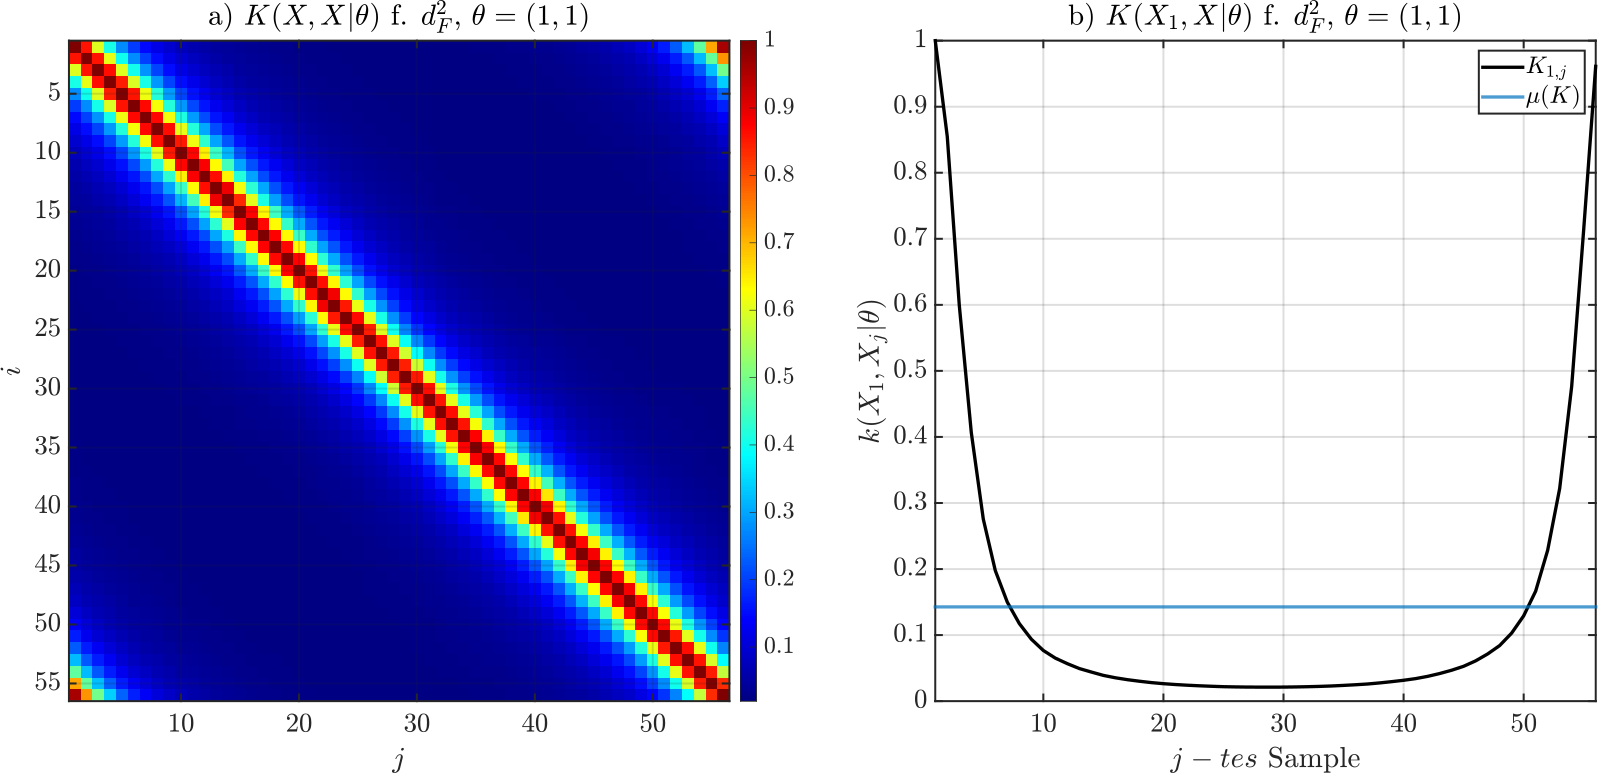
\includegraphics[width=\linewidth]{chapters/images/2-Grundlagen/Kernel-Vorabeiten-N56}
	\caption[Kernel-Implementierung der Vorarbeiten]{Kernel-Implementierung der Vorarbeiten, mittels Kovarianzfunktion $k(X_i,X_j)$ nach \autoref{eq:kfun} f. $d_F^2$ nach \autoref{eq:df2} und einen Trainingsdatensatz $X$ mit $N_{Ref} = 56$ gleich verteilten Simulationswinkeln $X_i \mapsto \alpha_i$. Die Skalierung durch Kernel-Parameter ist mit $\theta = (1,1)$ ausgeschaltet. In a) ist \autoref{alg:kmatrix} f. $K(X,X|\theta)$ genutzt und alle Trainingsdaten $X$ somit gegenseitig referenziert. Abbildung b) zeigt, Kovarianzen $K_{1,j}$ des Teildatensatz $X_1$, gegenüber sich selbst und jeden weiteren Satz $X_j$. Der Matrix-Mittelwert $\mu(K)$ in b), ist als Indikator über die gegenseitige Beeinflussung Datensätze im Regressionsverfahren zu interpretieren. Der genutzte Trainingsdatensatz $X$ basiert auf, gemachter TMR-Sensor \cite{TDK2016} Charakterisierung in \autoref{ch:tdk-datensatz}. Grafik nachempfunden aus \cite{Lang2014}}
	\label{fig:kernel-vorabeiten-n56}
\end{figure}


\clearpage


Ab hier folgt ein Wechsel der Notation um Bezüge zur Fachliteratur \cite{Rasmussen2006} zeigen zu können. Die veränderte Schreibweise ist im \autoref{sec:gprinit} unter Trainings- bzw. Testdatensätze zusammengefasst und beschrieben.
\newline
Die Parametrierung des Regressionsverfahren ist bisher empirisch ermittelt worden und stellt einen Angelpunkt in dieser Arbeit dar. Für eine selbstständige Optimierung, von Modellparametern und verbundener Modellgeneralisierung, müssen entsprechende Kriterien gebildet werden. Diese sind, in genutzter Literatur, als Minimierungsprobleme beschrieben \cite{Rasmussen2006}\cite{Guerrero2014}\cite{Lang2014}. 
\newline
Im Gegensatz zur Leitliteratur \cite{Rasmussen2006}, die Lösungsansätze für Regressionen eindimensionaler Funktionen beschreibt, ist für die Winkelvorhersage eine kombinierte Regression einer zweidimensionalen Funktion herzustellen. Da Ableitungen von Winkelstellungen, über orthogonal zueinander stehenden, Cosinus- und Sinus-Funktionen erfolgen. Dabei ist die Adaption der Array-Daten-Formate aus \autoref{sec:prinzip-des-sensor-arrays}, bereits in den Vorarbeiten gelöst worden \cite{Schuethe2020} und über die Kovarianzfunktion \autoref{eq:kfun} für $d_F^2$ \autoref{eq:df2} implementiert. \autoref{fig:kernel-vorabeiten-n56} zeigt die Implementierung aus den Vorarbeiten, anhand der Kovarianzfunktion und resultierender Kovarianzmatrix, für ein Beispiel eines $N_{Ref} = 56$ Observierungen großen Trainingsdatensatz. Für diese Implementierungsform, wäre das ein viel zu großer Datensatz in der realen Anwendung. In Bezug auf das Sensor-Array \autoref{sec:prinzip-des-sensor-arrays}, müssten $2 \times 56 = 112$ Matrizen abgelegt werden, sodass diese dem Regressionsprozess als Referenzen zur Verfügung stehen. Was hier zwar ein drastisches Beispiel ist, dass allerdings sehr schön das Verhalten der Kovarianz in Verbindung mit TMR basierten Daten zeigt.
\newline
Die Kovarianzfunktion mit resultierender Kovarianzmatrix, muss in der Lage sein systemische Eigenschaften wiedergeben zu können. Auf den TMR-Sensor \cite{TDK2016} gemünzt, muss die Matrix einfach periodisch sein. Das ist durch Kurvenverlauf in \autoref{fig:kernel-vorabeiten-n56} b) und durch ansteigenden Ecken links unten und rechts oben in a) zu erkennen. Es gibt nur eine vollwertige Diagonale. Bei Systemen höherer Periodizität, müsste die Kovarianzfunktion, entsprechend mehrere dieser Diagonalen, durch Superposition oder Trigonometrie-Funktionen erzeugen \cite{Rasmussen2006}.


\clearpage


Die homogenen Bereiche der Matrix zeigen, dass die Trainingsdaten $X$ mit gleichbleibender magnetischer Stimulanz erzeugt wurden. Gäbe es Fehllagen in der Erzeugung, Sprunghaften Versatz des Sensor-Arrays, oder Verkippung des Magneten, wären die Flächen unterbrochen. Ebenfalls indiziert die durchgehende Diagonale, dass die Rotation konstant mit gleichbleibenden Abständen vollzogen worden ist. Würden Sprünge in der Rotation auftauchen, müssten diese durch Schnitte in der Diagonale und eventuell durch Absenkungen der Ecken ersichtlich werden. Durch Bruch in der Periodizität würden Ecken der Matrix ganz verschwinden.


Der annähernd keilförmige Kurvenverlauf in \autoref{fig:kernel-vorabeiten-n56} b), bei ausgeschalteter Skalierung $\theta = (1,1)$, weißt auf ein System mit einfacher Komplexität hin \cite{Rasmussen2006}. Das heißt, es benötigt entweder eine erhöhte Anzahl von Trainingssamples, oder eine Parameteroptimierung und aufbohren der Modellkomplexität, um von den Trainingsdaten abweichende Daten, mit geringen Regressionsvarianzen prozessieren zu können \cite{Rasmussen2006}. Andersherum gesagt, gibt man alle möglichen in Winkelpositionen über die Trainingsdaten vor, muss der Regressionsfehler automatisch gegen null gehen. Die Modellanpassung auf eingespeiste Trainingsdaten, sowie gleichzeitige und sinnvolle Verringerung des Datenumfangs, bilden dabei die zu haltende Balance in Bezug auf akzeptable Winkelfehler \cite{Rasmussen2006}. 

 

